\documentclass[a4paper,10pt]{report}

\usepackage{tikz}
\usetikzlibrary{shadows.blur}
\usetikzlibrary{shapes.symbols}

\usepackage{fancybox, graphicx}
\usepackage{hyperref}
\usepackage{amsmath}
\usepackage{amssymb}
\usepackage{xspace}
\pagestyle{headings}
%\usepackage[margin=1.2in]{geometry}
\usepackage[left=2cm, right=2cm, top=2.5cm, bottom=2cm]{geometry}
\usepackage{float}
\restylefloat{table}
\usepackage{listings}
\usepackage{color}
\definecolor{gray}{rgb}{0.4,0.4,0.4}
\definecolor{darkblue}{rgb}{0.0,0.0,0.58}
\definecolor{attributeColor}{rgb}{0.96,0.517,0.29}
\definecolor{darkgreen}{rgb}{0,.392,0}
\definecolor{stringColor}{rgb}{0.6,0.2,0}
\usepackage{array,multirow}
\usepackage{longtable}
\usepackage{cleveref}
\usepackage{bbding}
\crefname{section}{�}{��}
\Crefname{section}{�}{��}
\usepackage[utf8]{inputenc}
\usepackage{tablefootnote}
\usepackage{algorithmic}
\usepackage{makecell}
\usepackage{multicol}

\usepackage{caption} 
\captionsetup[table]{skip=5pt}
\captionsetup[longtable]{skip=5pt}
\captionsetup[figure]{skip=1pt}

\usepackage[utf8]{inputenc}
\usepackage[english]{babel}
 
\newcounter{example}[section]
\newenvironment{example}[1][]{\refstepcounter{example}\par\medskip
   \textbf{Example~\theexample. #1} \rmfamily}{\medskip}
   
\newcounter{note}[section]
\newenvironment{note}[1][]{\refstepcounter{note}\par\medskip
   \textbf{Note~\thenote. #1} \rmfamily}{\medskip}
   
\newcommand{\myStartLine}{\par
  \kern8pt % space above the rules
  \hrule height 0.5pt
  \kern3pt % space below the rules
}
\newcommand{\myEndLine}{\par
  \kern3pt % space above the rules
  \hrule height 1.5pt
  \kern12pt % space below the rules
}

%\lstset{
%  basicstyle=\ttfamily,
%  columns=fullflexible,
%  showstringspaces=false,
%  commentstyle=\color{gray}\upshape
%  numbers=left,
%%  frame = single, 
%%  stepnumber=5
%}

\newcommand{\HRule}{\rule{\linewidth}{0.5mm}}

\lstdefinelanguage{XML}
{
  basicstyle=\ttfamily\footnotesize,
  morestring=[b]",
  morestring=[s]{>}{<},
  moredelim=[s][\bfseries\color{darkblue}]{<}{\ },
  moredelim=[s][\bfseries\color{darkblue}]{</}{>},
  moredelim=[l][\bfseries\color{darkblue}]{/>},
  moredelim=[l][\bfseries\color{darkblue}]{>},
  morecomment=[s]{<?}{?>},
  morecomment=[s]{<![CDATA[}{]]>},
  moredelim=[s][\bfseries\color{darkgreen}]{<!--}{-->},
  commentstyle=\color{darkgreen},
  stringstyle=\color{stringColor},
  identifierstyle=\color{red},
  keywordstyle=\color{attributeColor},
  morekeywords={oid,columnId,columnIdRef,symbId,symbolType,op,columnNum,columnType,
  valueType,inputTarget,blkId,blkIdRef,symbIdRef,xmlns,version,type,VariableMapping,
  IndividualMapping,schemaLocation,xs,xsi,NONMEMdataSet,matrixType,opType,order,
  math,ct,ds,mdef,mstep,mml,un,name,definition,writtenVersion,id,inputType,oidRef,catId,
  length,default,vectorIndex,diagDefault,offDiagDefault,row,column,numbRows,numbCols,
  dataSymbol,modelSymbol,ordered,compartmentNo,compNo,ordered,linkFunction,varId,
  censoringType,dataSymbol,modelSymbol,MarkovOrder,deviationMatrixType,implementedBy,
  argument,admNumber,transformId,transformIdRef,catIdRef} % list your attributes here
}


\newcommand{\cellml}{CellML\xspace}
\newcommand{\sbml}{SBML\xspace}
\newcommand{\sedml}{SED-ML\xspace}
\newcommand{\mathml}{MathML\xspace}
\newcommand{\uncertml}{UncertML\xspace}
\newcommand{\pml}{PharmML\xspace}
\newcommand{\pharmml}{PharmML\xspace}
\newcommand{\xelem}[1]{\texttt{<#1>}\index{XML Element!\texttt{<#1>}}}
\newcommand{\xatt}[1]{\texttt{#1}\index{XML Attribute!\texttt{#1}}}

\begin{document}

\begin{titlepage}
\begin{center}

% Upper part of the page. The '~' is needed because \\
% only works if a paragraph has started.

\includegraphics[width=0.35\textwidth]{./logo/ddmore_logo}~\\[1cm]

%\textsc{\LARGE }\\[1.5cm]
%
\textsc{\Large Internal Release}\\[0.5cm]

% Title
\HRule \\[0.4cm]
{ \huge \bfseries Extensions in PharmML 0.7 \\[0.4cm] }

\HRule \\[1.5cm]

% Author and supervisor
\begin{minipage}{0.5\textwidth}
\begin{flushleft} \large
\emph{Authors:}\\
Maciej J \textsc{Swat}\\
Pierre \textsc{Grenon}\\
Florent \textsc{Yvon}\\
Sarala \textsc{Wimalaratne}\\
Niels Rode \textsc{Kristensen}\\
\end{flushleft}
\end{minipage}
\begin{minipage}{0.4\textwidth}
\begin{flushright} \large
\emph{with contributions from:} \\
%%Roberto \textsc{Bizzotto} \\
Emmanuelle \textsc{Comets}\\
Paolo \textsc{Magni}\\
Lorenzo \textsc{Pasotti}\\
%Nadia \textsc{Terranova}\\
%%Marc \textsc{Lavielle}
\end{flushright}
\end{minipage}

\vfill
\begin{figure}[htb]
\centering
  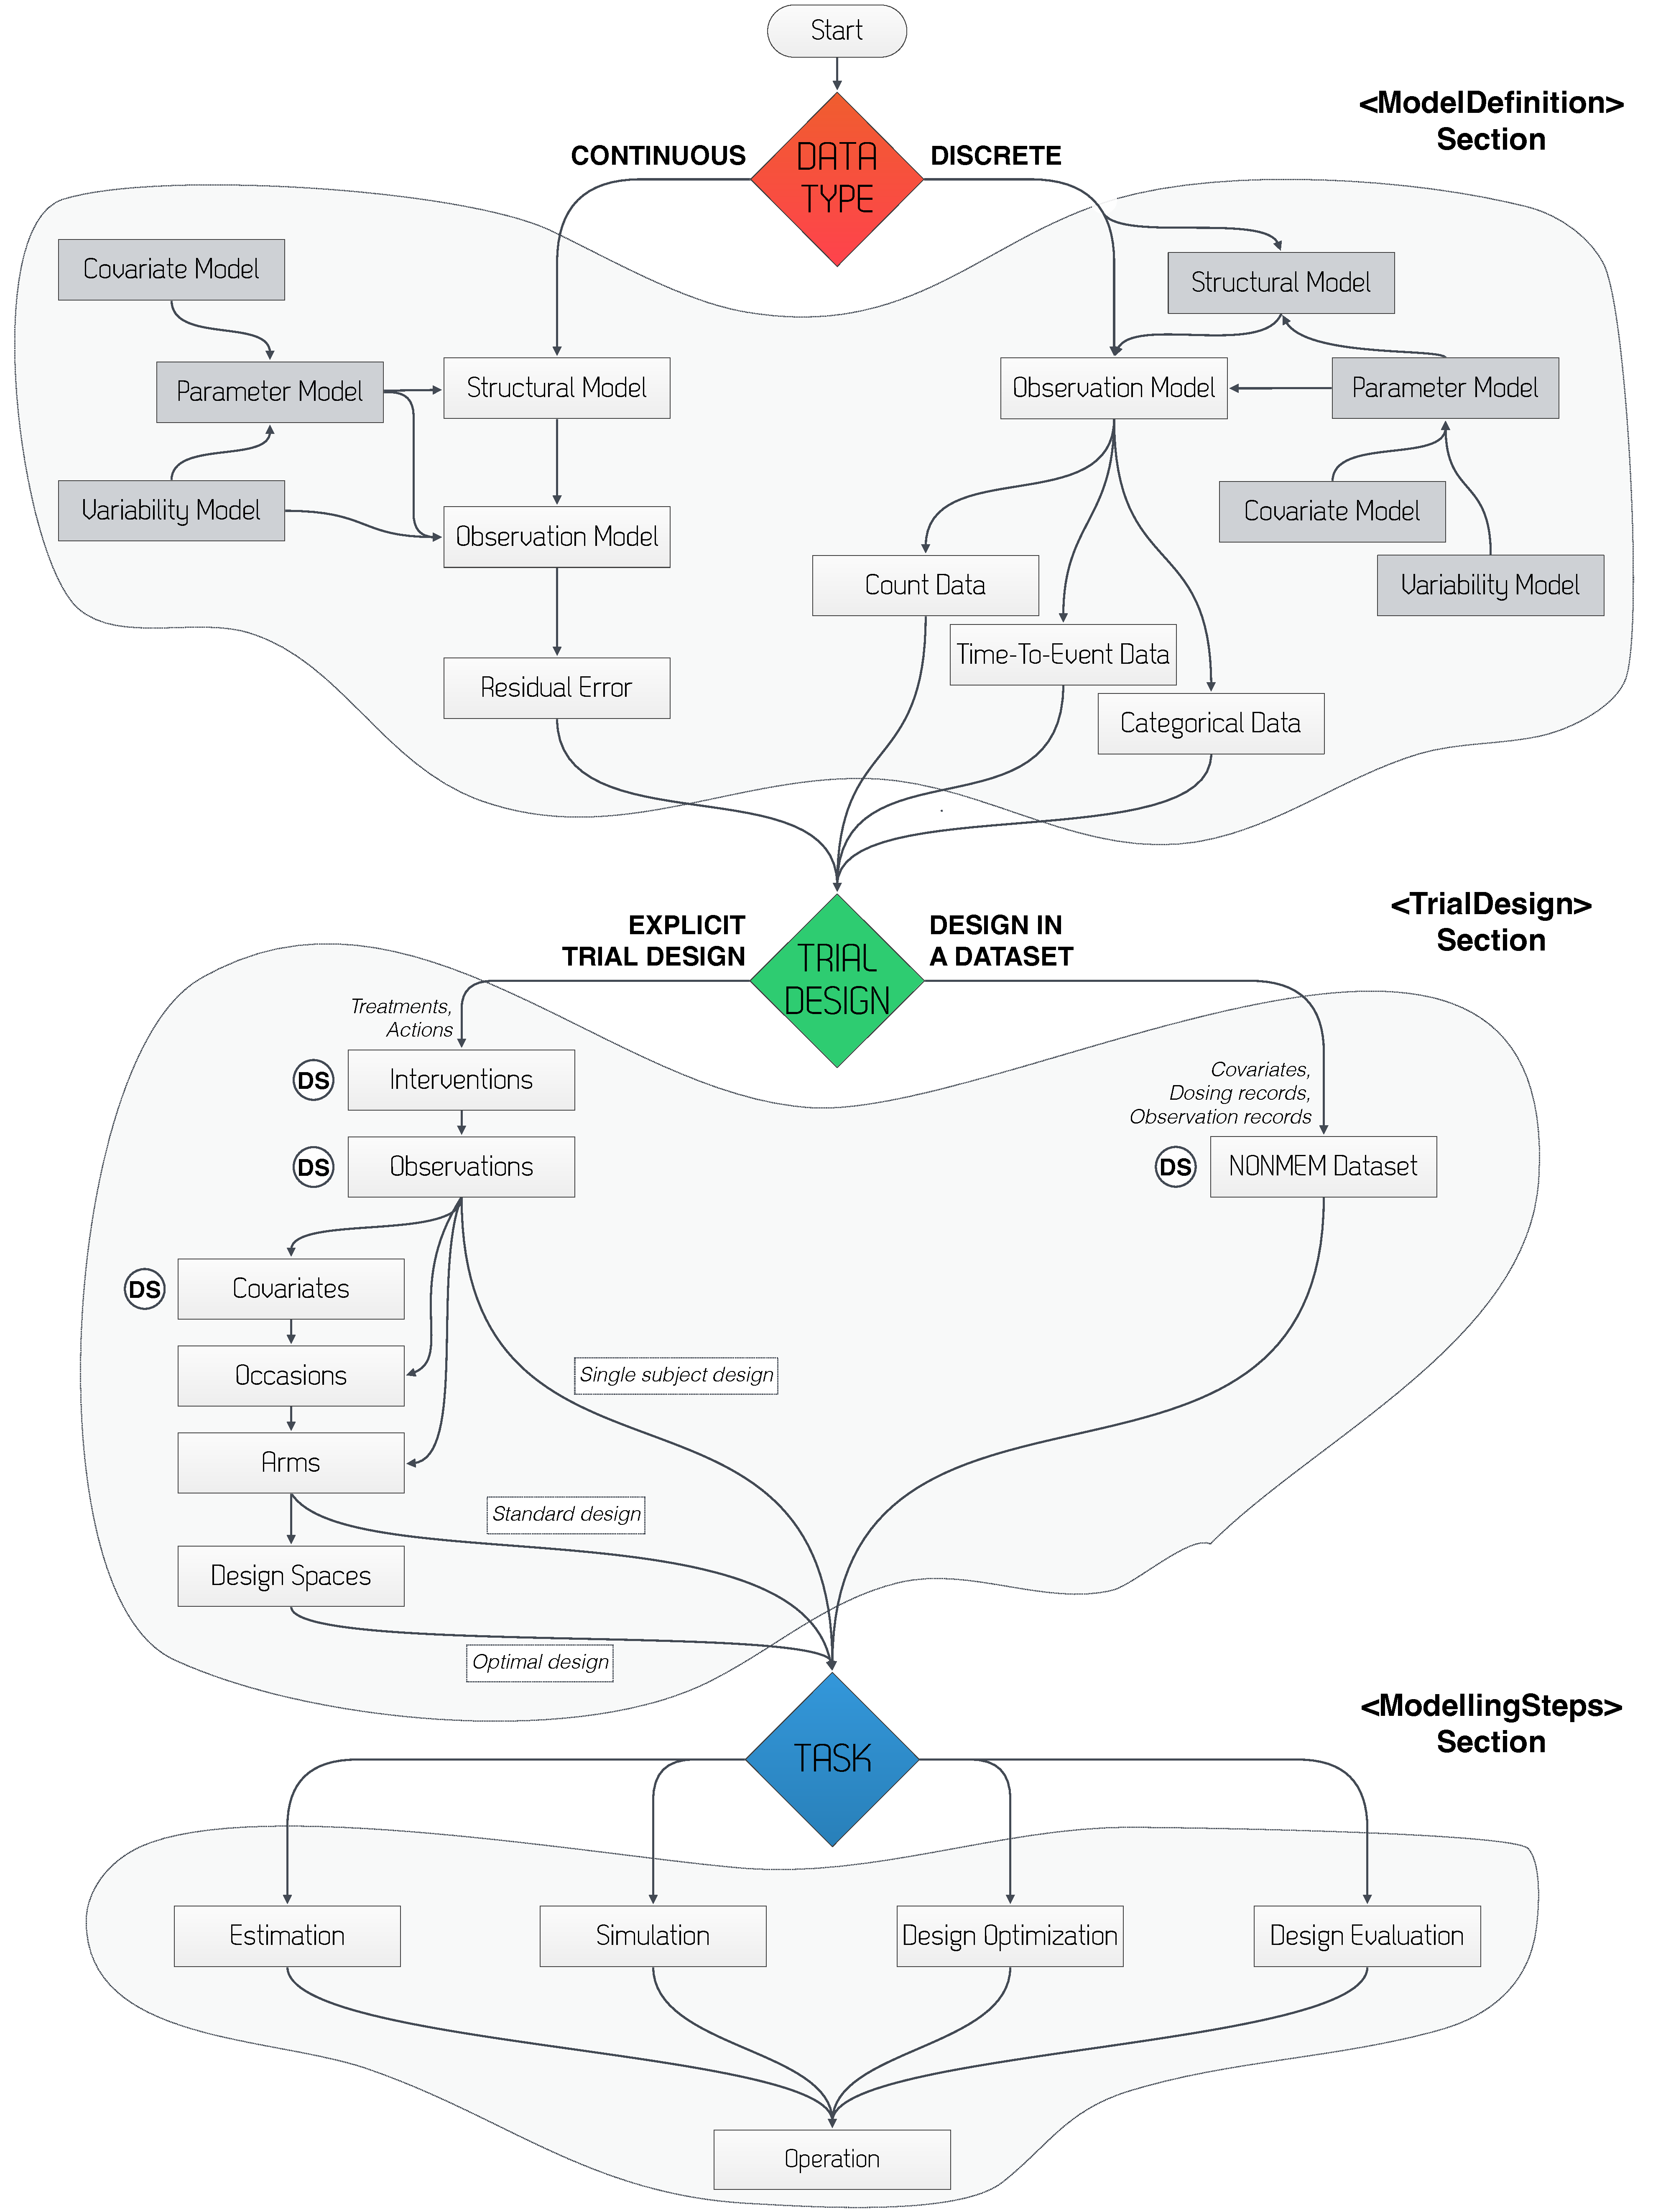
\includegraphics[width=90mm]{pics/Flowchart07}
\end{figure}



\vfill

% Bottom of the page
{\large \today \\}

\end{center}
\end{titlepage} 
	
%\maketitle

\tableofcontents


%%%%%%%%%%%%%%%%%%%%%%%%%%%%%%%%%%%%%%%%%%%%%%%%%%%%%%%%%%%%%%%%%%%%%%
%%%%%%%%%%%%%%%%%%%%%%%%%%%%%%%%%%%%%%%%%%%%%%%%%%%%%%%%%%%%%%%%%%%%%%%
%%%%%%%%%%%%%%%%%%%%%%%%%%%%%%%%%%%%%%%%%%%%%%%%%%%%%%%%%%%%%%%%%%%%%%%
%%%%%%%%%%%%%%%%%%%%%%%%%%%%%%%%%%%%%%%%%%%%%%%%%%%%%%%%%%%%%%%%%%%%%%%
\chapter{Overview}

This document describes extensions and changes in \pml compared to the
previously released version 0.


\section{Major changes/extensions in version 0.7 - under construction}
The following table summarises the changes described in detail in ...

\LTcapwidth=\textwidth
\begin{center}
%\renewcommand{\arraystretch}{1.1}%
\begin{longtable}{lll}
\hline
\hline
\pml element 				&  version $\le$ 0.6 				& version 0.7 \\
or modelling aspect 			& 							& \\
\hline
\hline
  \multicolumn{3}{c}{\textit{ProbOnto}}		\\
\hline
\hline
Probability distributions		& \uncertml used for encoding of 	& {\color{red} \scshape{new}} \xelem{Distribution} element with  \\
						& distributions					& children \xelem{ProbOnto} and \xelem{UncertML} \\
\hline
\emph{ProbOnto} - ontology and	&  	--					& -- support for expressions as parameters \\
knowledge base of			& 							& -- support for many related distribution \\
probability distribution 		& 							& functions and quantities \\
						&							& -- additional discrete and continues \\
						&							& distributions \\
\hline
\hline
  \multicolumn{3}{c}{\textit{MODELS}}		\\
\hline
\hline
'Distribution' type model 		& not available					& can be used with either \uncertml or \\
for covariates, parameters 	&							& ProbOnto \\
and observations			&							& \\
\hline
Individual parameter model	& 3 types supported: 'Equation'	& 4 types supported now \\
						& type, Gaussian with linear/ 		& -- \xelem{GaussianModel} extended to the generic  \\
						& nonlinear covariate model		& \xelem{StructuredModel} with linear/nonlinear \\
						&							& covariate model {\color{red} \scshape{modified}}\\
						&							& -- 'Equation' type (no changes) \\
						&							& -- {\color{red} \scshape{new}} 'Distribution' type model using  \\
						&							& either UncertML or ProbOnto \\
\hline
Population parameter		& \xelem{SimpleParameter} used	& \xelem{PopulationParameter} element {\color{red} \scshape{new}} \\	
						& with no distribution support		& \xelem{SimpleParameter} element removed \\
						&							& and replaced by \xelem{PopulationParameter}\\			
\hline
Covariate model			& Transformation, interpolation  	& Support for conditional distributions \\
						& and distribution of covariates 	& wrt covariates or design elements {\color{red} \scshape{new}} \\
						& supported					& \\
\hline
Matrix/Vector operators		& not supported				& Added inverse, trace and transpose \\
						&							& operators {\color{red} \scshape{new}} \\
\hline
\hline
  \multicolumn{3}{c}{\textit{BAYESIAN/HIERARCHICAL}}	\\
\hline
\hline
\hline
\hline
  \multicolumn{3}{c}{\textit{TRAIL DESIGN}}  \\
\hline
\hline
Lookup table 				& Available in \xelem{Administration}	& Moved to \xelem{Observations} \\
\hline
\hline
  \multicolumn{3}{c}{\textit{GENERAL}}  \\
\hline
\hline
Interval					& not available					& Element \xelem{Interval} with left/right- \\
						&							& endpoints of closed/open \xatt{type} attribute. \\
						&							& \xatt{closed} is the default value. \\
\hline
\caption{Overview of major differences between versions 0.7 and 0.6}
\label{figTable:overviewTable}
\vspace{-2em}
\end{longtable}
\end{center}


%\paragraph{Covariate model}
%Covariate model is barely covered so far. See also \cite{Keizer:2011aa}. Missing are following features:\\
%For categorical covariates:\\
%-- categorical distribution of categorical covariates \\
%---- estimating categorical distribution from external data file -- TEST \\
%---- sampling from known categorical distribution -- TEST \\
%---- clusters of categorical covariates \\
%For continuous covariates:\\
%-- power-normal distribution for continuous covariates \\
%---- estimating parameters $\lambda$,$\mu$,$\sigma$ from external data file \\
%---- sampling from known power-normal distribution \\
%---- conditional distribution of continuous covariates - DONE \\
%---- selecting criteria for continuous covariates \\
%---- dependent distribution of continuous covariates \\
%---- correlated continuous covariates \\
%For both types: \\
%-- selection/exclusion criteria missing \\


%%%%%%%%%%%%%%%%%%%%%%%%%%%%%%%%%%%%%%%%%%%%%%%%%%%%%%%%%%%%%%%%%%%%%%
%%%%%%%%%%%%%%%%%%%%%%%%%%%%%%%%%%%%%%%%%%%%%%%%%%%%%%%%%%%%%%%%%%%%%%%
%%%%%%%%%%%%%%%%%%%%%%%%%%%%%%%%%%%%%%%%%%%%%%%%%%%%%%%%%%%%%%%%%%%%%%%
%%%%%%%%%%%%%%%%%%%%%%%%%%%%%%%%%%%%%%%%%%%%%%%%%%%%%%%%%%%%%%%%%%%%%%%
\chapter{\emph{ProbOnto} -- Ontology/Knowledge Base of Probability Distributions}
\label{ch:ProbOnto}


\paragraph{Background}
The initial motivation for \emph{ProbOnto} was to create an ontology of probability 
distributions purely for annotation purposes. Many resources are available online 
and in printed format -- but no proper ontology exists so far\footnote{For 
example, the Statistics Ontology, STATO, \url{http://stato-ontology.org/}, provides 
for most distributions merely a link to an external reference/definition. No parameters
or related functions and quantities are defined in the ontology making their annotation
impossible. Other ontologies are setup in a similar way.}. 

When encoding probabilistic uncertainties the name of distribution of interest and 
its parameters are sufficient and in most cases such parameter set is unique. 
However, because for a number of cases two or more parameterisations exist, 
one needs to be careful what parameters are being used when referring to or 
encoding a distribution.

Until now, we have been relying on the UncertML standard \cite{uncertml3:2014}, 
which provides means to encode in MDL/PharmML a range of continuous and 
discrete uni/multi-variate probability distributions. However it has several limitations 
as described in the next section. 

\paragraph{Idea} It turns out that \emph{ProbOnto} can be very helpful in
designing a flexible alternative for UncertML with many additional features.
It can be used e.g. in PharmML or other target tools/languages \emph{both} 
as ontological resource for annotation purposes and as a knowledge base to 
provide the means to specify a wide range of distributions and several distribution 
related functions and quantities.

Such alternative solution is indispensable in the face of requirements 
posted by models we would like to encode currently and in foreseeable future. 

\section{Ontology versus Knowledge Base}
\begin{description}
\item[Ontology] is a formal representation of a domain of knowledge. It is an abstract entity 
defining the vocabulary for a domain and the relations between concepts.
However, an ontology doesn't specify how that knowledge is stored 
(as physical file, in a database, or in some other form), and how the knowledge 
can be accessed.
\item[Knowledge base] is a physical artifact. It is a database, a repository of information 
that can be accessed and manipulated in some predefined fashion.
\end{description}
The knowledge in a knowledge base is modelled according to rules and relationships 
defined in an ontology. \marginpar{\HandCuffLeft} 

%%%%%%%%%%%%%%%%%%%%%%%%%%%%%%%%%%%%%%%%%%%%%%%%%%%%%%%%%%%%%%%%%%%%%%
\section{Limitations of UncertML}
Although very useful to a certain extend, its design and scope has 
limitations making the encoding of some probability distribution cumbersome 
or impossible. Here some known limitations (in the order of severity):
\begin{itemize}
\item
it doesn't support the assignment of expression for distribution parameters.
\item
it doesn't support the specification of block references, which is required if the 
parameter in question is defined elsewhere in the model.
\item
it doesn't cover many distributions used in Pharmacometrics, e.g. 
\begin{itemize}
\item 
multivariate continues distributions such as Inverse-Wishart
\item
discrete distributions such as Generalized Poisson, Zero-inflated Poisson etc.
\item
or alternative parameterisations for distributions such 
as Negative Binomial, Log-Normal etc.
\end{itemize}
\item
\xelem{degreesOfFreedom} parameter element of the Wishart distribution doesn't support
referencing a variable (required for Bayesian inference) -- a known bug/limitation 
but with no solution for now.
\item
UncertML is only a reference resource for distributions and does not provide 
mechanisms to retrieve programmatically distribution related functions and
quantities.  
\end{itemize}
Other minor issues:
\begin{itemize}
%\item
%changes/updates in the unpublished version 3.0 happen without providing 
%documentation change-log.
\item
the implementation of \xelem{MultivariateNormalDistribution} requires the specification 
of the \xatt{dimension} attribute of the covariance matrix -- although this can be estimated
it requires unnecessary calculations when translating models to PharmML. 
\item
every extension requires changes in the XML schema -- comparable effort is much
lower for \emph{ProbOnto}.
\item
version 3.0 which we currently use is not yet released publicly, the UncertML website 
is not updated and 3.0 documentation is not available.
\end{itemize}

\paragraph{Suggested way forward} ProbOnto offers an alternative solution allowing
avoiding all the limitations listed above while providing number of additional features
and means to build in a very flexible probability distribution support in MDL and PharmML 
and other languages/tools within DDMoRe and beyond.

%%%%%%%%%%%%%%%%%%%%%%%%%%%%%%%%%%%%%%%%%%%%%%%%%%%%%%%%%%%%%%%%%%%%%%
\section{ProbOnto Features}
\begin{itemize}
\item
General 
\begin{itemize}
\item
covers almost 50 distributions and alternative parameterisations 
\item
supports encoding of mixture distributions and truncation bounds (open/closed)
\item
allows for easy encoding of distributions and related functions in target tools/languages 
due to its generic format
\item
doesn't enforce specific implementation in target tool 
\item
in PharmML only few extensions were required to provide flexible encoding support
for all distributions and their features
\item
collection of supported distributions is easily extendable without impact 
on PharmML structure
\item
mathematical functions and quantities are encoded in Latex, plain text 
representation is planned  
\end{itemize}
\item
ProbOnto as Ontology
\begin{itemize}
\item
it can be used to annotate statistical models based on a known probability distribution, 
e.g. their name, parameters, truncation bounds, their defining functions and quantities 
\end{itemize}
\item
ProbOnto as Knowledge Base
\begin{itemize}
\item
provides for each distribution either PDF or PMF and in many cases also 
other distribution related functions such as CDF, Hazard and Survival functions 
-- the level of coverage depends on the particular distribution
\item
provides related quantities such as mean, median, mode etc.
\item
provides other info about support and relationships to other distributions
\end{itemize}
\end{itemize}
The distribution collection and their features are based, among others, on \cite{Forbes:2010jk},
\cite{Leemis:2008tg}, \cite{}, \cite{}, \cite{}

%%%%%%%%%%%%%%%%%%%%%%%%%%%%%%%%%%%%%%%%%%%%%%%%%%%%%%%%%%%%%%%%%%%%%%
\subsection{Features under construction}
The following features are under construction and not available in the current 
release. They are available to certain extend in UncertML, which should be used
for the time being if required.
\begin{itemize}
\item
truncation bounds -- supported for univariate distributions already 
but an extension to multivariate distributions is need.
%\item
%mixture models - added but more testing required -- see example 'Poisson with mixture distribution', PMIX.
\item
non-parametric distributions.
\end{itemize}



%%%%%%%%%%%%%%%%%%%%%%%%%%%%%%%%%%%%%%%%%%%%%%%%%%%%%%%%%%%%%%%%%%%%%%%
\section{Alternative parameterisations -- examples}
Following the request to cover alternative parameterisations for normal/log-normal
distribution, \emph{ProbOnto} provides these, used by modellers or required by our target 
tools.

\subsection{Negative binomial distribution}
Available parameterisations are
\begin{itemize}
\item
NegativeBinomial1\,($r$, $p$) with r -- \emph{number of failures} and p -- \emph{success probability},
\begin{align}
P(y=k;r,p) = \binom {k+r-1}k (1-p)^r p^k \nonumber
\end{align}
\item
NegativeBinomial2\,($\lambda$, $\tau$) with $\lambda$ -- \emph{Poisson intensity} and $\tau$ -- \emph{over-dispersion},
\begin{align}
P(y=k;\lambda,\tau) = \frac{\Gamma(k + \frac{1}{\tau})}{k!\; \Gamma(\frac{1}{\tau})} \Big(\frac{1}{1+\tau \lambda} \Big)^{\frac{1}{\tau}} 
\Big(\frac{\lambda}{\frac{1}{\tau} + \lambda} \Big)^{k} \nonumber
\end{align}
\end{itemize}
with the latter being used in typical pharmacometric discrete data models, \cite{Plan:2009fk, Troconiz:2009fv}.
\subsection{Normal distribution}
Available parameterisations, see Table \ref{figTable:logNormalParameterisations} for the 
defining probability density functions, are
\begin{itemize}
\item
Normal1\,($\mu$, $\sigma$) with $\mu$ -- \emph{mean} and $\sigma$ -- \emph{standard deviation}, 
\item
Normal2\,($\mu$, \emph{var}) with $\mu$ -- \emph{mean} and \emph{var} -- \emph{variance},
\item
Normal3\,($\mu$, $\tau$) with $\mu$ -- \emph{mean} and $\tau$ -- \emph{precision} ($\tau=1/\sigma^2$)
\end{itemize}

\begin{center}
\small
\renewcommand{\arraystretch}{1.1}%
\begin{longtable}{llcccc}
  \hline
  \hline
\multicolumn{1}{c}{\textbf{ProbOnto}}& Paramete- 	& \textbf{UncertML} 	& \textbf{WinBUGS}	& \textbf{Monolix} & \textbf{NONMEM} \\
\multicolumn{1}{c}{0.2}			& risation		&  3.0			& 1.4		& 4.3	& 7.3 \\
  \hline
Negative Binomial 1	& \textit{r}, \textit{p}	&	y	&	y	& y  &  -- \\
Negative Binomial 2 	& $\lambda, \tau$ & --  & --  & --  &  -- \\[0.5ex]
Log-Normal 1	& $\mu$, $\sigma$	&	y	&	--	&	y	&  -- \\
Log-Normal 2	& $\mu$, \textit{var}	&	y	&	--	&	y	&  -- \\
Log-Normal 3	& \textit{m}, $\sigma$	&	--	&	--	&	--	&  -- \\
Log-Normal 4	& \textit{m}, \textit{cv}		& 	--	&	--	&	--	&  -- \\
Log-Normal 5	& $\mu$, $\tau$		& 	--	&	y	&	--	&  -- \\[.5ex]
Normal 1	& $\mu, \sigma$	&	y	&	--	&	y	& y  \\
Normal 2	& $\mu, var$	&	y	&	--	&	y	&  y \\
Normal 3	& $\mu, \tau$		&	--	&	y	&	--	&  -- \\
Standard Normal & $\mu=0, \sigma=1$	& -- & -- &	 y & y (CDF)  \\[0.5ex]
  \hline \\
\caption{Few univariate distributions with multiple parameterisations. Note that  in
many cases, the DDMoRe target tools uses different parameterisation.}
\label{figTable:NormalLogNormal}
\vspace{-3.5em}
\end{longtable}
\end{center}

\begin{figure}[htb!]
\centering
\begin{tabular}{cc}
% \includegraphics[width=140mm]{pics/CDF_17Dec} \\
 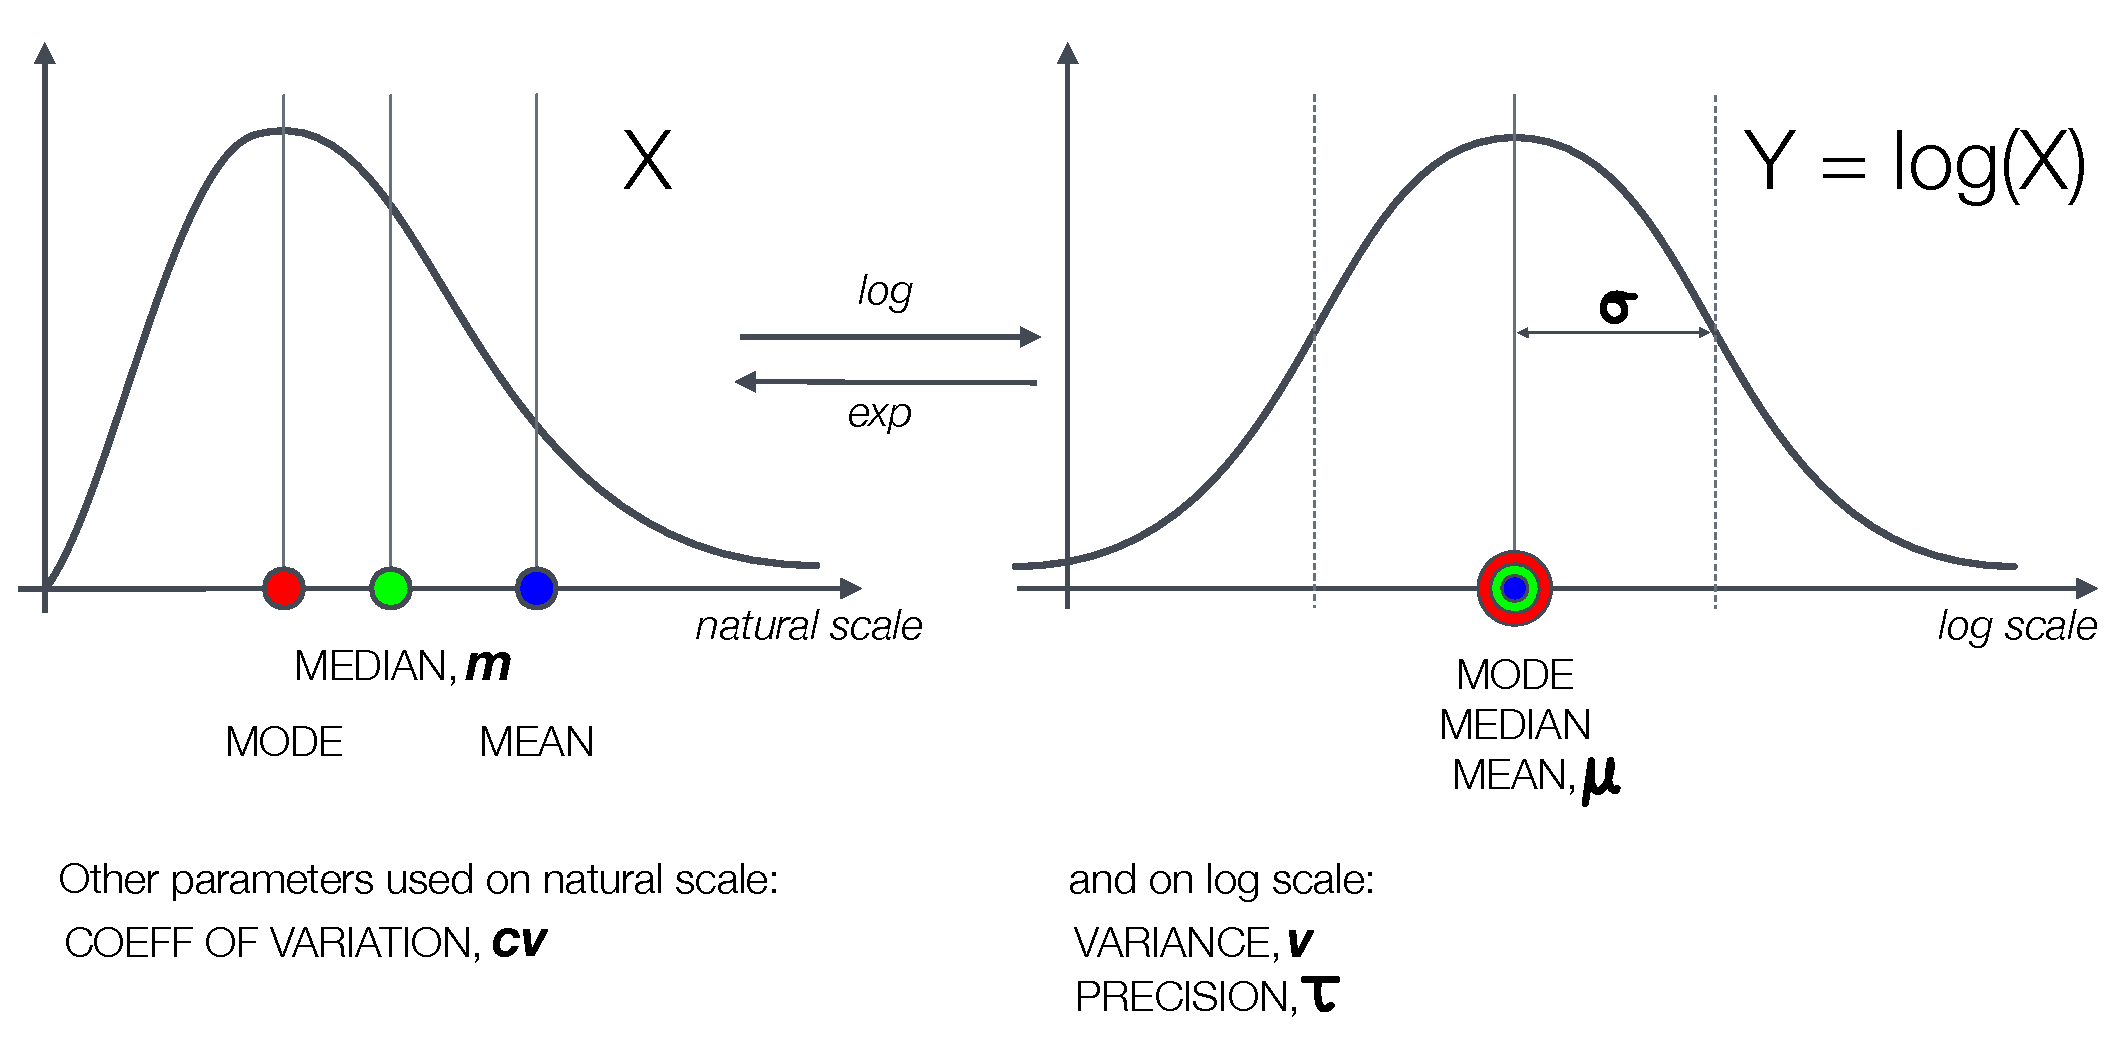
\includegraphics[width=140mm]{pics/normalAndLogDomain_schema}
\end{tabular}
\caption{Schematic representation of the lognormaly distributed data on the natural (left) 
and logarithmic scale (right), see Figure \ref{fig:insulinData} for real-life data example. 
\textbf{Bold} symbols stand for available quantities to parameterise a log-normally distributed 
variable.}
\label{fig:schematicLogNormal}
\end{figure}

\subsection{Log-normal distribution}
The log-normal distribution is special in that not only different parameter sets exist
but also they are defined either on the natural or logarithmic scale and in one case 
the parameters are defined on these two different scales, see Figure \ref{fig:schematicLogNormal},
for an overview.\\
Available parameterisations (also listed in Table \ref{figTable:NormalLogNormal} 
with indication about their coverage in target tools) are 
\begin{itemize}
\item
LogNormal1\,($\mu$, $\sigma$) with \emph{mean}, $\mu$, and \emph{standard deviation}, $\sigma$, both on the log-scale, 
\item
LogNormal2\,($\mu$, \textit{var}) with \emph{mean}, $\mu$, and \emph{variance}, $var$, both on the log-scale, 
\item
LogNormal3\,(\textit{m}, $\sigma$)  with \emph{median}, $m$, on the natural scale and \emph{standard deviation}, $\sigma$, on the log-scale, 
\item
LogNormal4\,(\textit{m}, \textit{cv}) with \emph{median}, $m$, and \emph{coefficient of variation}, $cv$, both on the natural scale, 
\item
LogNormal5\,($\mu$, $\tau$) with \emph{mean}, $\mu$, and \emph{precision}, $\tau$, both on the log-scale.
\end{itemize}

\begin{figure}[htb!]
\centering
\begin{tabular}{cc}
 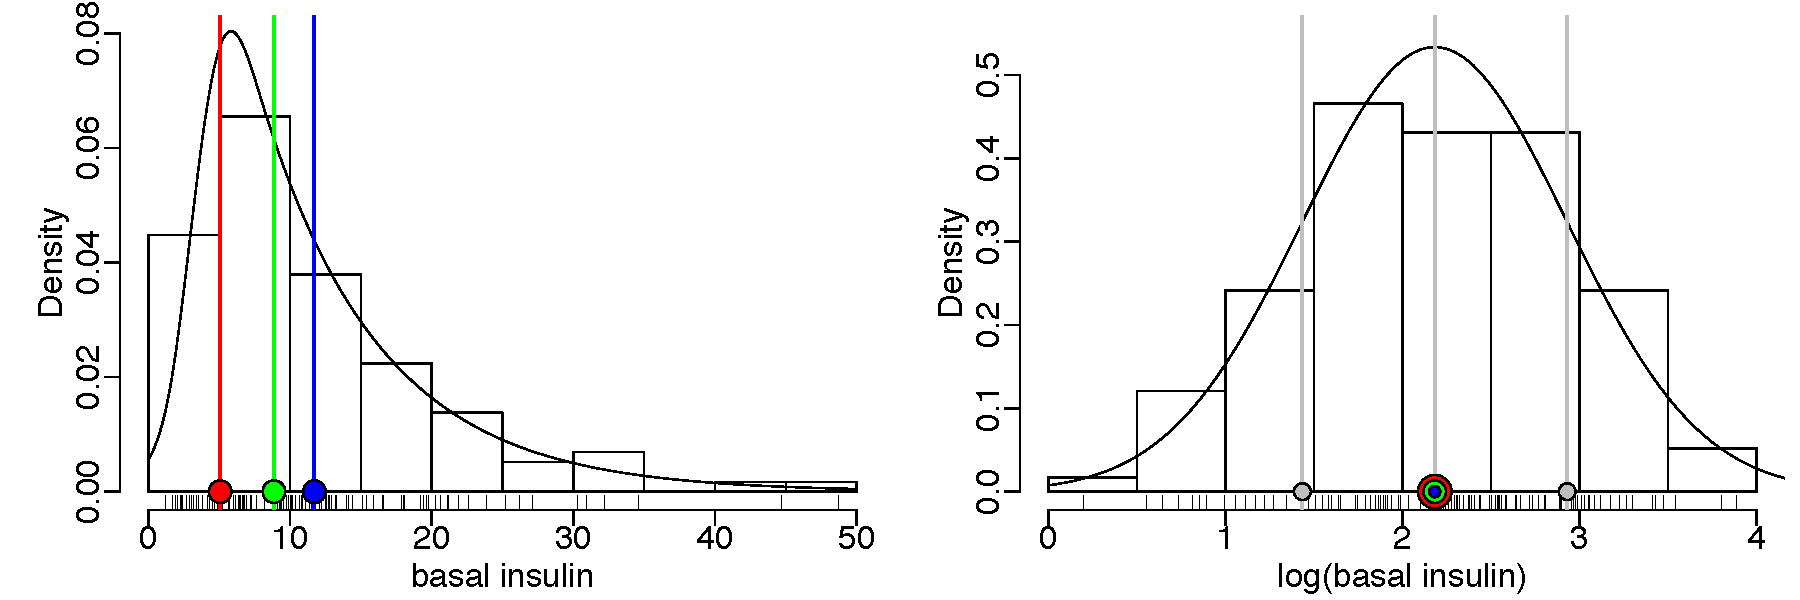
\includegraphics[width=140mm]{pics/normalAndLogDomain}
\end{tabular}
\caption{Representation of the lognormaly distributed basal insulin data in diabetic patients 
\cite{Rudenski:1991aa} on the natural scale (left) and on the logarithmic scale after 
$log$--transformation (right), colour code as in Figure \ref{fig:schematicLogNormal}. 
The density estimation for the data on the natural scale and its plotting was performed 
using the R package \textit{logspline} \cite{Kooperberg:2013}.}
\label{fig:insulinData}
\end{figure}


\cleardoublepage
\setlength{\tabcolsep}{2em}

\LTcapwidth=.9\textwidth
\begin{center}
\small
\renewcommand{\arraystretch}{1}%
\begin{longtable}{ccc}
 \hline
 \hline
\multicolumn{1}{c}{Log-normal distribution} 	& \multirow{2}{*}{Quantity} 	&\multicolumn{1}{c}{Normal distribution on the} \\ [-.5ex]
\multicolumn{1}{c}{on the natural scale (NS)} 	&						& \multicolumn{1}{c}{log-transformed scale (LS)} \\
   \hline
  \hline
  \multicolumn{3}{c}{$LN1: P(x;\boldsymbol\mu,\boldsymbol\sigma)=\Gape[.5cm][.3cm]{} \frac{1}{x \sigma \sqrt{2 \pi}} \exp\Big[ \frac{-(\log x - \mu)^2}{2\sigma^2}\Big] $ }\\
   \hline
$e^{\mu + \frac{1}{2}\sigma^2}$			& \Gape[.4cm][0cm]{}Mean  	& $\boldsymbol\mu$ \\ [.15ex]
$e^{2\mu + \sigma^2}[e^{\sigma^2}-1]$		& Variance 				& $\sigma^2$	\\ [.15ex]
\multirow{2}{*}{$e^{\mu + \frac{1}{2}\sigma^2}\sqrt{e^{\sigma^2}-1}$} & Standard	& \multirow{2}{*}{$\boldsymbol\sigma$}	\\ [-.5EX]
									& deviation  				&		 	\\ [.15ex]
 $e^{\mu - \sigma^2}$	 				& Mode 					&	 $\mu$	\\ [.15ex]
\multirow{2}{*}{$e^\mu$}					& \multirow{2}{*}{Median}		& \multirow{2}{*}{$\mu$} \\ [-.5EX]
									&						& \\[.15ex]
\multirow{2}{*}{$\sqrt{e^{\sigma^2}-1}$}		& Coefficient 				&   \multirow{2}{*}{$\sigma/\mu$} \\ [-.5EX]
									& of variation				& \\
  \hline
  \multicolumn{3}{c}{$LN2: P(x;\boldsymbol\mu,\boldsymbol {v})=\Gape[.5cm][.3cm]{} \frac{1}{x \sqrt{v} \sqrt{2 \pi}} \exp\Big[ \frac{-(\log x - \mu)^2}{2 v}\Big] $ }\\
   \hline
$e^{\mu + \frac{1}{2}v}$					& \Gape[.4cm][0cm]{}Mean  	& $\boldsymbol\mu$ \\ [.15ex]
$e^{2\mu + v}[e^{v}-1]$					& Variance 				& $\boldsymbol v$	\\ [.15ex]
\multirow{2}{*}{$e^{\mu + \frac{1}{2} v}\sqrt{e^{v}-1}$} 	& Standard		& \multirow{2}{*}{$ {\sqrt{v}}$}	\\ [-.5EX]
									& deviation  				& 	\\ [.15ex]
$e^{\mu - v}$	 						& Mode 					& $\mu$	\\ [.15ex]
\multirow{2}{*}{$e^\mu$	}				& \multirow{2}{*}{Median}		& \multirow{2}{*}{$\mu$} \\ [-.5EX]
									&						& \\[.15ex]
\multirow{2}{*}{$\sqrt{e^{v}-1}$}			& Coefficient 				& \multirow{2}{*}{$ {\sqrt{v}} /\mu$} \\ [-.5EX]
									& of variation				& \\
  \hline
  \multicolumn{3}{c}{$LN3: P(x;\boldsymbol m,\boldsymbol \sigma) =\Gape[.5cm][.3cm]{} \frac{1}{x \sigma \sqrt{2 \pi}} \exp\Big[ \frac{-[\log(x/m)]^2}{2\sigma^2}\Big] $ }\\ %[1.5EX]
   \hline
 $m\, e^{\frac{1}{2}\sigma^2}$				& \Gape[.4cm][0cm]{}Mean  	& $\log( m)$ \\ [.15ex]
 $m^2 e^{\sigma^2} [e^{\sigma^2}-1]$		& Variance 				& $\sigma^2$	\\ [.15ex]
 \multirow{2}{*}{$m\sqrt{e^{\sigma^2} (e^{\sigma^2}-1)}$}	& Standard  	& \multirow{2}{*}{$\boldsymbol\sigma$}	\\ [-.5EX]
									& deviation  				& 	\\ [.15ex]
 $m/e^{\sigma^2}$	 					& Mode 					& $\log( m)$	\\ [.15ex]
 $\boldsymbol m$						& Median 					& $\log( m)$	\\ [.15ex]
  \multirow{2}{*}{$\sqrt{e^{\sigma^2}-1}$	}	& Coefficient				& \multirow{2}{*}{$\sigma/\log( m)$} \\ [-.5EX]
 									&  of variation				&  \\
  \hline
   \multicolumn{3}{c}{$LN4: P(x;\boldsymbol m,\boldsymbol {cv})=\Gape[.5cm][.3cm]{} \frac{1}{x \sqrt{\log(cv^2+1)} \sqrt{2 \pi}} \exp\Big[ \frac{-[\log(x/m)]^2}{2\log(cv^2+1)}\Big] $} 	\\
   \hline
 $m \log(cv^2 + 1)$						& \Gape[.4cm][0cm]{}Mean  	& $\log( m)$ \\ [.15ex]
 $m \,(cv^2+1)\,cv^2$					& Variance 				& $\log(cv^2 + 1)$	\\ [.15ex]
 \multirow{2}{*}{$\sqrt{m\,(cv^2+1)}\,cv$}		& Standard  				& \multirow{2}{*}{$\sqrt{\log(cv^2 + 1)}$}	\\ [-.5EX]
 									& deviation  				& 	\\ [.15ex]
 $m / (cv^2 + 1)$	 					& Mode 					& $\log( m)$	\\ [.15ex]
 $\boldsymbol m$						& Median 					& $\log( m)$	\\ [.15ex]
 \multirow{2}{*}{$ {\boldsymbol {cv}}$}		& Coefficient 				& \multirow{2}{*}{$\sqrt{\log(cv^2 + 1)}/\log( m)$} \\ [-.5EX]
 									& of variation				&  \\
  \hline
  \multicolumn{3}{c}{$LN5: P(x;\boldsymbol\mu,\boldsymbol \tau)=\Gape[.5cm][.3cm]{} \sqrt{\frac{\tau}{2 \pi}} \frac{1}{x} \exp\Big[ {-\frac{\tau}{2}(\log x-\mu)^2} \Big] $ }\\
   \hline
 $e^{\mu + \frac{1}{2\tau}}$				& \Gape[.4cm][0cm]{}Mean  	& $\boldsymbol\mu$ \\ [.15ex]
 $e^{2\mu + \frac{1}{\tau}}[e^{\frac{1}{\tau}}-1]$	& Variance 			& $1/\tau$	\\ [.15ex]
\multirow{2}{*}{$e^{\mu + \frac{1}{2} \frac{1}{\tau}}\sqrt{e^{\frac{1}{\tau}}-1}$} 	& Standard	& \multirow{2}{*}{$\sqrt{1/\tau}$}	\\ [-.5EX]
									& deviation  				& 	\\ [.15ex]
 $e^{\mu - \frac{1}{\tau}}$					& Mode 					& $\mu$	\\ [.15ex]
\multirow{2}{*}{$e^\mu$	}				& \multirow{2}{*}{Median}		& \multirow{2}{*}{$\mu$} \\ [-.5EX]
									&						& \\[.15ex]
\multirow{2}{*}{$\sqrt{e^{\frac{1}{\tau}}-1}$}	& Coefficient 				& \multirow{2}{*}{$\sqrt{1/\tau} / \mu$} \\ [-.5EX]
									& of variation				& \\
   \hline
\caption{Representation of the available parameterisations for the log-normal distribution. With
$\boldsymbol m$ -- scale parameter (NS), $\boldsymbol {cv}$ -- dispersion parameter (NS),
$\boldsymbol \mu$ -- location parameter (LS), $\boldsymbol \sigma$ -- scale parameter (LS),
$\boldsymbol v$ -- scale parameter (LS). See Figure \ref{fig:schematicLogNormal} for 
the meaning of the symbols.}
%$\boldsymbol \sigma$ -- shape parameter }
\label{figTable:logNormalParameterisations}
\vspace{-3.5em}
\end{longtable}
\end{center}

\setlength{\tabcolsep}{1em}

\newpage 

\LTcapwidth=.95\textwidth
\begin{center}
\small
\renewcommand{\arraystretch}{1.1}%
\begin{longtable}{llcccc}
  \hline
  \hline
\multicolumn{1}{c}{\textbf{ProbOnto}}& Paramete- 	& \textbf{UncertML} 	& \textbf{WinBUGS}	& \textbf{Monolix} & \textbf{NONMEM} \\
\multicolumn{1}{c}{0.2}			& risation		&  3.0			& 1.4		& 4.3	& 7.3 \\
  \hline
  \hline
  \multicolumn{6}{c}{\textit{Discrete Univariate}}  \\
  \hline
Bernoulli				& \emph{p}		&	y	&	y	& --  &  -- \\
Binomial				& \emph{n, p}		&	y	&	y	& --  &  -- \\
Categorical ordered		& \emph{k}, \{$p_1, \ldots, p_k$\}	& y	&	y	& --  &  -- \\
Categorical unordered	& \emph{k}, \{$p_1, \ldots, p_k$\}	&	y	&	y	& --  &  -- \\
Generalized Poisson	& $\lambda, \delta$	& --  & --  & --  &  -- \\
Geometric			& \emph{p}		&	y	& --  & --  &  -- \\
Hypergeometric		& \emph{N, K, n}	&	y	& --  & --  &  -- \\[0.5ex]
Negative Binomial 1		& \emph{r, p}		&	y	&	y	& --  &  -- \\
Negative Binomial 2 		& $\lambda, \tau$ 	& --  & --  & --  &  -- \\[0.5ex]
Poisson				& $\lambda$		&	y	&	y	& --  &  -- \\
%Poisson with 			&	& --  & --  & --  &  -- \\[-0.5ex]
%Markov elements 		&	& --  & --  & --  &  -- \\
%Poisson with			&	& --  & --  & --  &  -- \\[-0.5ex]
%mixture distribution 	&	& --  & --  & --  &  -- \\[0.5ex]
Uniform 1 (discrete)		&  \emph{a, b}		& --	& --	& -- & --  \\
Uniform 2 (discrete)		&  0, \emph{n}		& --	& --	& -- & --  \\[0.5ex]
Zero-inflated Poisson	& $\lambda, \pi$	& --  & --  & --  &  -- \\
  \hline
  \multicolumn{6}{c}{\textit{Continuous Univariate}}	\\
  \hline
Beta					& $\alpha, \beta$	&	y	&	y	&	y	&  -- \\
Cauchy				& $x_0, \gamma$	&	y	& --  & --  &  -- \\
Chi-squared			& \emph{k}		&	y	&	y	&	y	&  -- \\
%Dirac Delta			&	&	y	& --  & --  &  -- \\
Exponential			& $\lambda$		&	y	&	y	&	y	&  -- \\
F (aka Fisher-Snedecor)	& $d_1, d_2$		&	y	& --  &	y	&  -- \\
Gamma				& $k, \theta$		&	y	&	y	&	y	&  -- \\
Generalized Gamma	& \emph{a, d, p}	&	y	& --  & --  &	  \\
Gompertz				& $\eta, b$		& --  &	y	& --  &	  \\
Gumbel 				& \multirow{2}{*}{$\mu, \beta$}	& \multirow{2}{*}{--}  & \multirow{2}{*}{y} & \multirow{2}{*}{--}  &  \multirow{2}{*}{--} \\ [-0.5ex]
(aka Extreme Value) \\
Inverse-Gamma		& $\alpha, \beta$	&	y	& --  & --  &  -- \\	
Laplace 				& \multirow{2}{*}{$\mu, b$} &	\multirow{2}{*}{y}	&	\multirow{2}{*}{y}	& \multirow{2}{*}{--}  & \multirow{2}{*}{--} \\ [-0.5ex]
(aka Double-exponential) \\[0.5ex]
Log-Normal 1			& $\mu, \sigma$	&	y	&	--	&	y	&  -- \\
Log-Normal 2			& $\mu$, \textit{var}	&	y	&	--	&	y	&  -- \\
Log-Normal 3			& \emph{m}, $\sigma$	&	--	&	--	&	--	&  -- \\
Log-Normal 4			& \emph{m, cv}		& 	--	&	--	&	--	&  -- \\
Log-Normal 5			& $\mu$, $\tau$	& 	--	&	y	&	--	&  -- \\[0.5ex]
Logistic				& $\mu, s$		&	y	&	y	& --  &  -- \\[0.5ex]
Normal 1				& $\mu, \sigma$	&	y	&	--	&	y	& y  \\
Normal 2				& $\mu, var$		&	y	&	--	&	y	&  -- \\
Normal 3				& $\mu, \tau$		&	--	&	y	&	--	&  -- \\[0.5ex]
Normal-inverse-gamma	& $\mu, \lambda$	& y	& --  & --  &  -- \\
Pareto				& $x_m, \alpha$	& y	& y	& --  &  -- \\
Rayleigh				& $\sigma$		& --  & --  & y	&  -- \\
Standard Normal 		& $\mu=0, \sigma=1$	& y & -- &	 y & y*  \\
Student's T			& $\nu$			& y	& y	& y	&  -- \\
Uniform				&  \emph{a, b}		& y	& y	& y		& --  \\
Standard Uniform		& $a=0, b=1$		& --	& --	& y & y  \\
Weibull				& $\lambda, k$		& y	& y	& y	&  -- \\
   \hline \\
\caption{Univariate distributions supported in ProbOnto, version 0.2. 
See Appendix \ref{ch:probontoAppendix} for the detailed description 
of the essential distributions required for ongoing use cases 
-- full ProbOnto knowledge base will be released next. *CDF is also provided 
as the \emph{PHI} function, \cite{NONMEM:2009}.}
\label{figTable:univariates}
\end{longtable}
\end{center}

\newpage

\LTcapwidth=.95\textwidth
\begin{center}
\small
\renewcommand{\arraystretch}{1.1}%
\begin{longtable}{lllccc}
  \hline
  \hline
\multicolumn{2}{c}{\textbf{ProbOnto 0.2}}	& Paramete- 	& \textbf{UncertML} 	& \textbf{WinBUGS} \\
Long name 	& Code Name			& risation		&  3.0			& 1.4 \\
  \hline
  \hline
  \multicolumn{5}{c}{\textit{Discrete Multivariate}} \\
  \hline
Multinomial	& Multinomial &	 $n, p_1, \ldots, p_k$ &	y	&	y \\
  \hline
  \multicolumn{5}{c}{\textit{Continuous Multivariate}} \\
  \hline
Dirichlet	&Dirichlet	& $K, \alpha_1, \cdots, \alpha_K$	& y	& y \\
Inverse-Wishart	&InverseWishart	& $\boldsymbol \Psi, \nu$	& --  & --  \\[0.5ex]
Multivariate Normal	1 & MultivariateNormal1	& $\boldsymbol {\mu}, \boldsymbol \Sigma $	& y	& --	 \\
Multivariate Normal	2 & MultivariateNormal2	& $\boldsymbol {\mu}, \boldsymbol T $	& --	& y	 \\[0.5ex]
Multivariate (Student) T 1	& MultivariateStudentT1	& $\boldsymbol {\mu}, \boldsymbol \Sigma, \nu$	& y	& --	 \\
Multivariate (Student) T 2 & MultivariateStudentT2	& $\boldsymbol {\mu}, \boldsymbol T, \nu$ & --	& y	 \\[0.5ex]
Wishart	& Wishart	& $\boldsymbol V, n$	& y	& y	 \\
   \hline
\caption{Multivariate distributions. Monolix \& NONMEM have been omitted as neither
of them features a multivariate distribution in current versions (as of April 2015).
See the appendix for the detailed description of the 
most relevant distributions -- full ProbOnto database will be released next.}
\label{figTable:multivariates}
\vspace{-2.5em}
\end{longtable}
\end{center}


%%%%%%%%%%%%%%%%%%%%%%%%%%%%%%%%%%%%%%%%%%%%%%%%%%%%%%%%%%%%%%%%%%%%%%
\section{ProbOnto and discrete data models}
\label{sec:ProbOntoAndDiscrete}
\subsection{Encoding of nominal categorical data models}

Consider the following \emph{ObservationModel} for nominal categorical data:

\begin{itemize}
\item
Type of observed variable -- discrete/categorical
\item
Category variable: $y$
\item
Set of categories: $\{1,2,3\}$
\item
Probabilities for category '1' and '2'
\begin{eqnarray}
&& p2 := P(y=1) = a1/(a1+a2+a3)  \nonumber \\
&& p1 := P(y=2) = a2/(a1+a2+a3)  \nonumber 
\end{eqnarray}
\end{itemize}
The following code shows how to implement the model 
starting with the general information: parameters involved and equations
for the probabilities 
\lstset{language=XML}
\begin{lstlisting}
<CategoricalData ordered="no">
    <!-- can alternatively be defined as individual parameters with IIV etc.-->
    <PopulationParameter symbId="a1"/> 
    <PopulationParameter symbId="a2"/>
    <PopulationParameter symbId="a3"/>
    
    <PopulationParameter symbId="p1">
        <ct:Assign>
            <math:Equation>
                <math:Binop op="divide">
                    <ct:SymbRef symbIdRef="a1"/>
                    <math:Binop op="plus">
                        <ct:SymbRef symbIdRef="a1"/>
                        <math:Binop op="plus">
                            <ct:SymbRef symbIdRef="a2"/>
                            <ct:SymbRef symbIdRef="a3"/>
                        </math:Binop>
                    </math:Binop>
                </math:Binop>
            </math:Equation>
        </ct:Assign>
    </PopulationParameter>
    <PopulationParameter symbId="p2">
        <ct:Assign>
            <math:Equation>
                <math:Binop op="divide">
                    <ct:SymbRef symbIdRef="a2"/>
                    <math:Binop op="plus">
                        <ct:SymbRef symbIdRef="a1"/>
                        <math:Binop op="plus">
                            <ct:SymbRef symbIdRef="a2"/>
                            <ct:SymbRef symbIdRef="a3"/>
                        </math:Binop>
                    </math:Binop>
                </math:Binop>
            </math:Equation>
        </ct:Assign>
    </PopulationParameter>
\end{lstlisting}
then listing the categories 
\lstset{language=XML}
\begin{lstlisting}
    <ListOfCategories> 
        <Category symbId="cat1"/>
        <Category symbId="cat2"/>
        <Category symbId="cat3"/>
    </ListOfCategories>                    
    <CategoryVariable symbId="y"/>
\end{lstlisting}
and eventually defining the unordered categorical distribution, \emph{CategoricalNonordered} in ProbOnto,
with 
\begin{itemize}
\item 
1st parameter  -- number of categories, here equal 3
\item 
2nd parameter  -- event probabilities vector, $p_1, \ldots, p_k$
\end{itemize}

\lstset{language=XML}
\begin{lstlisting}
    <PMF linkFunction="identity">
        <Distribution>
            <ProbOnto>
                <DistributionName>CategoricalNonordered</DistributionName>
                <!-- number of categories -->
                <Parameter order="1">
                    <ct:Assign>
                        <ct:Int>3</ct:Int>
                    </ct:Assign>
                </Parameter>
                <!-- event probabilities - a vector of length 2 -->
                <Parameter order="2">
                    <ct:Assign>
                        <ct:Vector>
                            <ct:VectorElements>
                                <ct:SymbRef symbIdRef="p1"/>
                                <ct:SymbRef symbIdRef="p2"/>
                            </ct:VectorElements>
                        </ct:Vector>
                    </ct:Assign>
                </Parameter>
            </ProbOnto>
        </Distribution>
    </PMF>
</CategoricalData>
\end{lstlisting}
For the last second parameter, given there are $k$ categories, by default the 
specification of $k-1$ probabilities is sufficient assuming $\Sigma p_i = 1$.
Note that alternatively, the expressions for $p1$ and $p2$ could be used directly 
as \xelem{VectorElements}.


\subsection{Zero-inflated Poisson -- ZIP}
ProbOnto simplifies the encoding of the discrete models significantly. 
So far unavailable distributions such as Generalized Poisson (GP), 
Zero-inflated Poisson (ZIP) and others frequently used in pharmacometrics,
\cite{Plan:2009fk, Troconiz:2009fv}, are now easily encodable. The following example illustrates that.

The essential elements of the model are the following PMF
\[
\begin{cases}
  \log(P(Y=k)) = \log(1-p0) - \lambda + k\log(\lambda) - factln(k) 	& \text{ if } k > 0 \\
  \log(P(Y=k)) = \log(p0 + (1-p0)\exp(-\lambda)) 				& \text{else}
\end{cases}
\]
and the definition of model parameters, the Poisson intensity, $\lambda$,
and the probability of extra zeros, $p0$. In the case of explicitly encoded PMF
the model becomes lengthly as the following code illustrates which comes always 
with a risk of unnecessary misspelling. 

\subsubsection{Explicitly encoded ZIP model}
\lstset{language=XML}
\begin{lstlisting}
<ObservationModel blkId="om1">
    <Discrete>
        <CountData>
            <PopulationParameter symbId="k"/>
            <CountVariable symbId="y"/>
            
            <IntensityParameter symbId="Lambda">
                <ct:Assign>
                    <ct:SymbRef blkIdRef="pm1" symbIdRef="lambda"/>
                </ct:Assign>
            </IntensityParameter>
            
            <ZeroProbabilityParameter symbId="P0">
                <ct:Assign>
                    <ct:SymbRef blkIdRef="pm1" symbIdRef="p0"/>
                </ct:Assign>
            </ZeroProbabilityParameter>
            
            <PMF linkFunction="log">
                <math:LogicBinop op="eq">
                    <ct:SymbRef symbIdRef="y"/>
                    <ct:SymbRef symbIdRef="k"/>
                </math:LogicBinop>
                <ct:Assign>
                    <math:Equation>
                        <math:Piecewise>
                        <!-- 50 lines of code skipped here -->
                        <!-- for encoding of the conditional PMF: -->
                        <!-- if (k > 0): log(1-p0)-lambda+k*log(lambda)-factln(k) -->
                        <!-- else: log(p0+(1-p0)*exp(-lambda)) -->
                        </math:Piecewise>
                    </math:Equation>
                </ct:Assign>
            </PMF>
        </CountData>
    </Discrete>
</ObservationModel>
\end{lstlisting}
        
        
\subsubsection{ZIP model encode using ProbOnto}
In contrast to the first option, encoding of known models suing ProbOnto
becomes very easy as the generic structure is used and only the distribution
name and parameters need to be specified.

\lstset{language=XML}
\begin{lstlisting}
<ObservationModel blkId="om1">
    <Discrete>
        <CountData>
            <CountVariable symbId="y"/>
            <NumberCounts symbId="k"/>
            
            <PMF linkFunction="log">
                <math:LogicBinop op="eq">
                    <ct:SymbRef symbIdRef="y"/>
                    <ct:SymbRef symbIdRef="k"/>
                </math:LogicBinop>
                <Distribution>
                    <ProbOnto>
                        <DistributionName>ZeroInflatedPoisson</DistributionName>
                        <!-- Poisson intensity -->
                        <Parameter order="1">
                            <ct:Assign>
                                <ct:SymbRef blkIdRef="pm1" symbIdRef="Lambda"/>
                            </ct:Assign>
                        </Parameter>
                        <!-- probability of extra zeros -->
                        <Parameter order="2">
                            <ct:Assign>
                                <ct:SymbRef blkIdRef="pm1" symbIdRef="P0"/>
                            </ct:Assign>
                        </Parameter>
                    </ProbOnto>
                </Distribution>
            </PMF>
        </CountData>
    </Discrete>
</ObservationModel>
\end{lstlisting}

\subsection{Poisson with mixtures -- PMIX}
Rather the creating specific types for Poisson with mixture distribution for individual 
observations (PMIX), described in the PharmML 0.6 spec, \cite{Pharmml_06},
\begin{eqnarray}
P(y_{ij} = k;\pi,\lambda_1,\lambda_2) &=& \pi \frac{e^{-\lambda_1} \lambda_1^k}{k!} + (1-\pi) \frac{e^{-\lambda_2} \lambda_2^k}{k!} \nonumber
\end{eqnarray}
with $\lambda_1, \lambda_2 > 0$ and $\pi \in [0,1]$
the generic \emph{MixtureDistribution} can be used as the following code shows.

\lstset{language=XML}
\begin{lstlisting}
        <PMF linkFunction="identity">
            <Distribution>
                <ProbOnto>
                    <DistributionName>MixtureModel</DistributionName>
                    <!-- mixture parameter -->
                    <Parameter order="1">
                        <ct:Assign>
                            <ct:SymbRef symbIdRef="pi"/>
                        </ct:Assign>
                    </Parameter>
                    <!-- 1st mixture component -->
                    <MixtureComponent>
                        <DistributionName>Poisson</DistributionName>
                        <Parameter order="1">
                            <ct:Assign>
                                <ct:SymbRef symbIdRef="lambda1"/>
                            </ct:Assign>
                        </Parameter>
                    </MixtureComponent>
                    <!-- 2nd mixture component -->
                    <MixtureComponent>
                        <DistributionName>Poisson</DistributionName>
                        <Parameter order="1">
                            <ct:Assign>
                                <ct:SymbRef symbIdRef="lambda2"/>
                            </ct:Assign>
                        </Parameter>
                    </MixtureComponent>
                </ProbOnto>
            </Distribution>
        </PMF>
\end{lstlisting}
with \xelem{MixtureComponent} encoding the mixtures in questions and \xelem{Parameter},
$\pi$, the mixture probability. 
The solution has the advantage to be extendable to any number
\paragraph{Discussion}
The use of a generic \emph{MixtureDistribution} seems justified in this case. 
However, because reference literature exists for general Mixed Poisson regression models, 
\cite{Wang:1996fj}, the introduction of such specialised mixture distribution 
could be considered for ProbOnto in future as well.


%%%%%%%%%%%%%%%%%%%%%%%%%%%%%%%%%%%%%%%%%%%%%%%%%%%%%%%%%%%%%%%%%%%%%%
%%%%%%%%%%%%%%%%%%%%%%%%%%%%%%%%%%%%%%%%%%%%%%%%%%%%%%%%%%%%%%%%%%%%%%%
%%%%%%%%%%%%%%%%%%%%%%%%%%%%%%%%%%%%%%%%%%%%%%%%%%%%%%%%%%%%%%%%%%%%%%%
%%%%%%%%%%%%%%%%%%%%%%%%%%%%%%%%%%%%%%%%%%%%%%%%%%%%%%%%%%%%%%%%%%%%%%%
\chapter{Parameter, Covariate, Observation Models}
\label{ch:Models}


%%%%%%%%%%%%%%%%%%%%%%%%%%%%%%%%%%%%%%%%%%%%%%%%%%%%%%%%%%%%%%%%%%%%%%
\section{Distribution type -- generic model type {\color{red} \scshape{new}}}
\label{sec:newModelType}
The new model follows the textbook notation for definition of the distribution 
of a random variable and can be applied for covariate, parameter, observation etc.
\begin{itemize}
\item
Distribution type -- using ProbOnto or UncertML
\begin{align*}
	h(X) & \sim distribution(parameter1, parameter2, \dots) 
\end{align*}
e.g. 
\begin{align*}
\log(X) & \sim \mathcal N\big(\log(X_{typical}), \omega_X\big)
\end{align*}
\end{itemize}
with X covariate, parameter, observation etc. Examples will be given below.


%%%%%%%%%%%%%%%%%%%%%%%%%%%%%%%%%%%%%%%%%%%%%%%%%%%%%%%%%%%%%%%%%%%%%%
\section{Individual parameter representations -- extended}
\label{sec:individualParameter}

Following changes have been introduced 
for broader class of parameter models
\begin{itemize}
\item
\xelem{GaussianModel} renamed to \xelem{StructuredModel}
\item
\xelem{PopulationParameter} renamed to \xelem{PopulationValue} for consistency
\item
\xelem{Transformation} element has been redesigned in order to account for
Box-Cox transformation (see Section \ref{sec:BoxCoxTrafo} for a description).
Instead of 
\lstset{language=XML}
\begin{lstlisting}
                <StructuredModel>
                    <Transformation>log</Transformation>
\end{lstlisting}
now it reads
\lstset{language=XML}
\begin{lstlisting}
                <StructuredModel>
                    <Transformation type="log"/>
                    ...
\end{lstlisting}
%\lstset{language=XML}
%\begin{lstlisting}
%            <IndividualParameter symbId="V">
%                <StructuredModel>
%                    <Transformation type="BoxCox">
%                        <Lambda>
%                            <ct:Assign>
%                                <ct:SymbRef symbIdRef="lambda"/>
%                            </ct:Assign>
%                        </Lambda>
%                    </Transformation>
%\end{lstlisting}


\end{itemize}

\begin{itemize}
\item
Type 1. Structured (e.g. Gaussian) model 
\begin{itemize}
\item
	A.  Linear covariate model
\begin{align*}
         	h(\psi_i) = h(\psi_{pop}) + \beta c_i + \eta_i \quad [\text{Gaussian if } \eta_i \sim N(.,.)]
 \end{align*}
               
\item
	B. General covariate model
\begin{align*}
        	h(\psi_i) = H(\beta, c_i) + \eta_i  \quad [\text{Gaussian if } \eta_i \sim N(.,.)]
\end{align*}
\end{itemize}

\item
Type 2. General model 
\begin{itemize}
\item
	A. Equation type
\begin{align*}
       		\psi_i = H(\beta, c_i, \eta_i)
\end{align*}
                
\item
      	B. (NEW) Distribution type (i.e. eta-free notation)
\begin{align*}
		& h(\psi_i) \sim Distribution(parameter1, parameter2, \dots) \\
		e.g.& \\
		&\log(\psi_i) \sim \mathcal N\big(\log(\psi_{pop}) + \beta c_i, \omega_{\psi}\big) 
%		##### ADD NOTE on time vayrying covariates
\end{align*}
\end{itemize}
\end{itemize}

\begin{example}
From hierarchical model as proposed by Marc Lavielle \cite{LavielleFourModels:2014}

\lstset{language=XML}
\begin{lstlisting}
            <!-- V = {distribution=logNormal, prediction=V_pred, sd=omega_V} -->
            <IndividualParameter symbId="V">
                <ct:VariabilityReference>
                    <ct:SymbRef blkIdRef="vm1" symbIdRef="indiv"/>
                </ct:VariabilityReference>
                <Distribution>
                    <UncertML>
                        <LogNormalDistribution xmlns="http://www.uncertml.org/3.0" definition="">
                            <logScale>
                                <var varId="V_pred"/>
                            </logScale>
                            <shape>
                                <var varId="omega_V"/>
                            </shape>
                        </LogNormalDistribution>
                    </UncertML>
                </Distribution>
            </IndividualParameter>
\end{lstlisting}
\end{example}

\begin{note} \xelem{StructuredModel} extends \xelem{GaussianModel} to a more general
without loosing the ability to express the later -- 
this updated element allows e.g. Student-T distributed parameters to be formulated in the additive form
\begin{align*}
                \log(V_i) = \log(V_{pop}) + \beta c_i + \eta_i, \quad \text{with} \quad \eta_i \sim StudentT(0,\omega_V)
\end{align*}
\end{note}

\begin{note}  New Distribution-type (Type 2B) allows using UncertML/ProbOnto 
to define model without the random effect detour, e.g.
\begin{align*}
		\log(V_i) \sim \mathcal N\big(\log(V_{pop}), \omega_V\big) 		
\end{align*}
which is equivalent to 
\begin{align*}
                \log(V_i) = \log(V_{pop}) + \eta_i \quad \text{with} \quad \eta_i \sim \mathcal N(0,\omega_V)
\end{align*}
\end{note}

\begin{note}   ProbOnot, compared to UncertML, provides additional support for 
expressions in parameters, e.g. $mean = log(V_{pop})$ in the above equation.
\end{note}

\begin{note} Type 2B comes with support for multiple levels of variability, Figure \ref{fig:IOVtree},
\begin{align*}
		\log(V_{ik}) \sim \mathcal N\big(\log(V_{pop}), \omega_V + \kappa_V\big)
\end{align*}
\end{note}

\begin{figure}[htb!]
\centering
 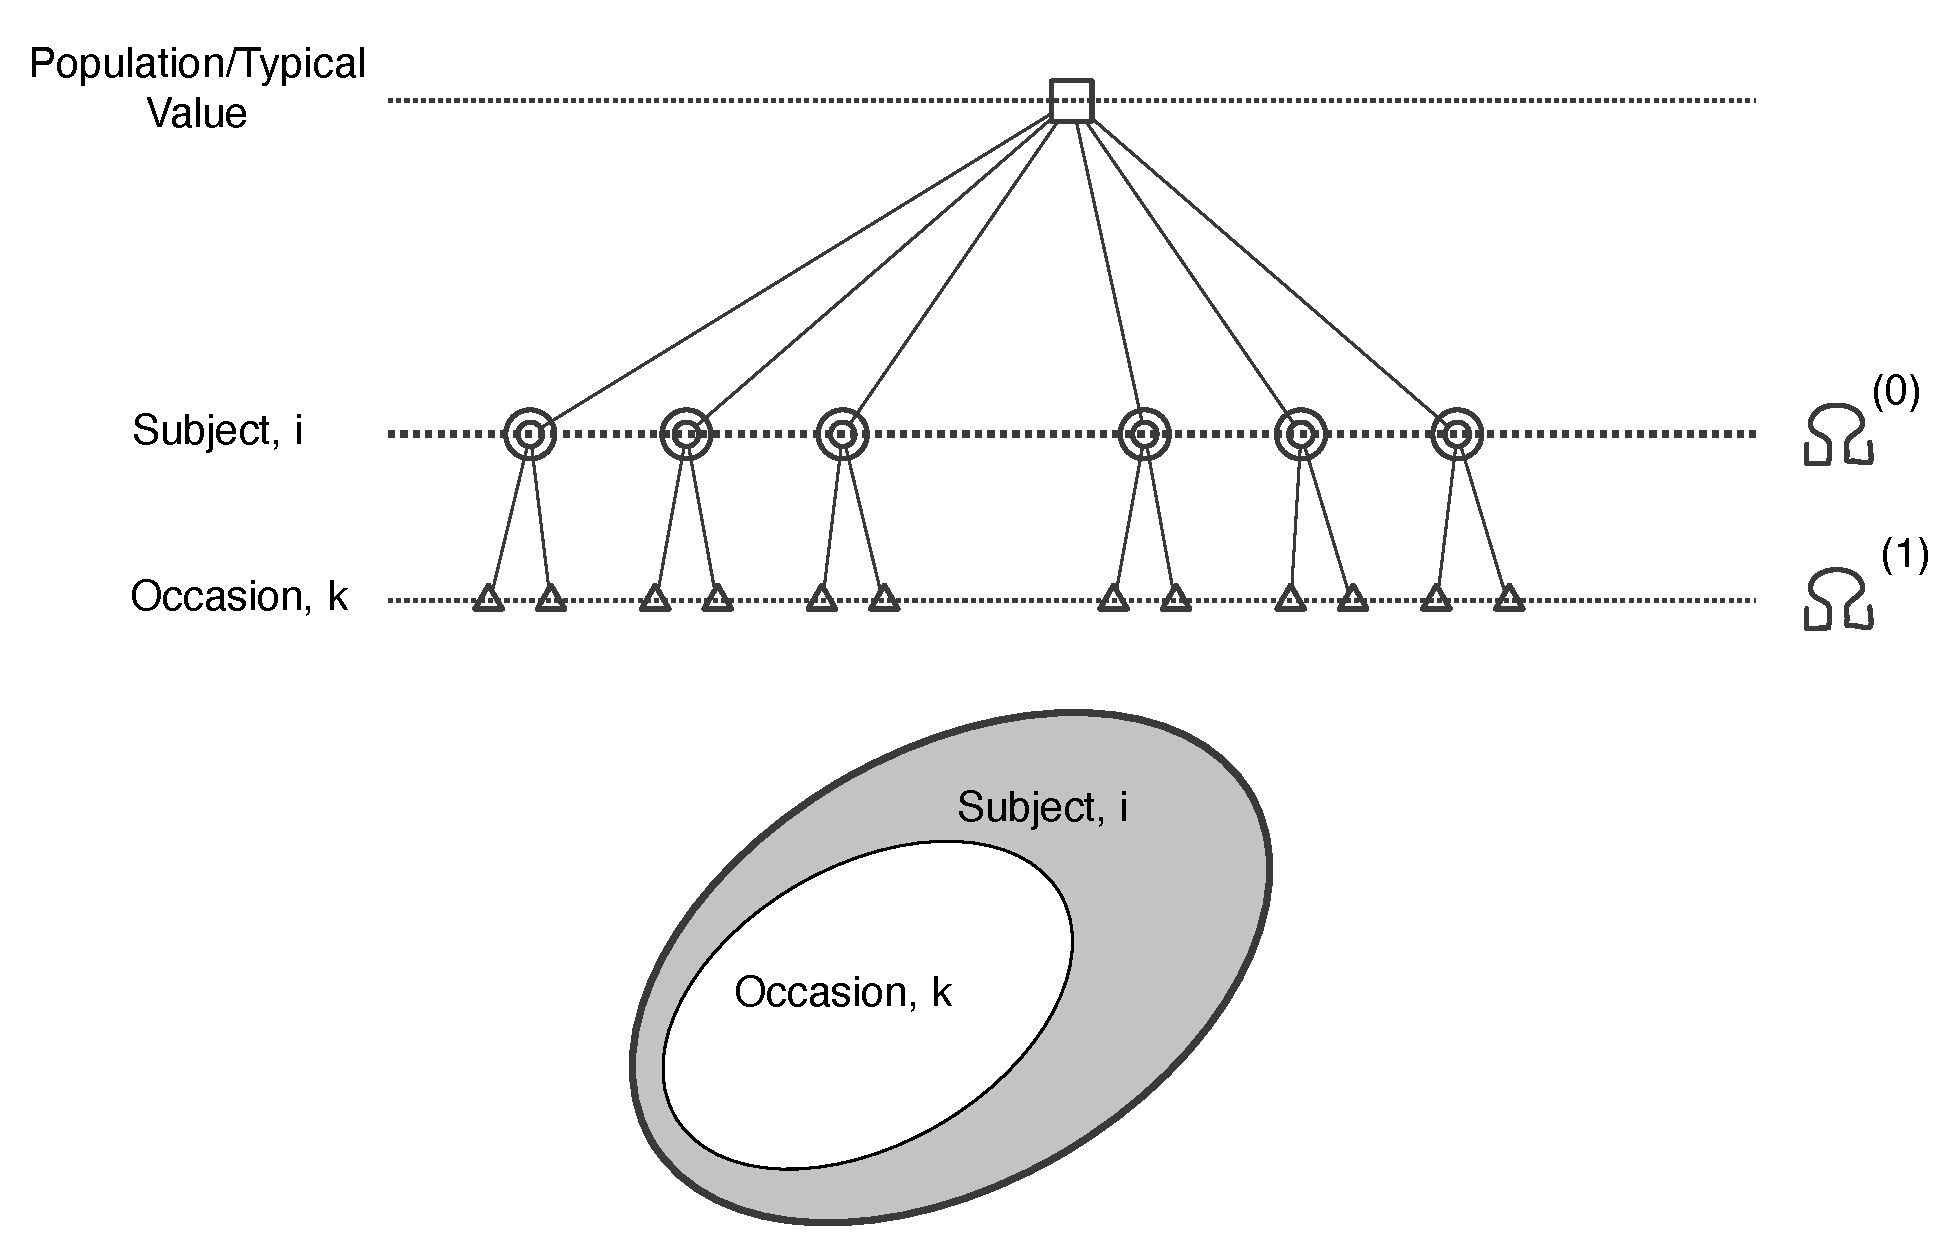
\includegraphics[width=120mm]{pics/IOV_2levels}
\caption{Model with IOV variability level.}
\vspace{-1em}
\label{fig:IOVtree}
\end{figure}


as the following PharmML snippet shows
\lstset{language=XML}
\begin{lstlisting}
            <IndividualParameter symbId="V">
                <ct:VariabilityReference>
                    <ct:SymbRef symbIdRef="iov"/>
                    <ct:RandomEffectMapping>
                        <ct:SymbRef symbIdRef="kappa_V"/>
                    </ct:RandomEffectMapping>
                </ct:VariabilityReference>
                <ct:VariabilityReference>
                    <ct:SymbRef symbIdRef="subject"/>
                    <ct:RandomEffectMapping>
                        <ct:SymbRef symbIdRef="omega_V"/>
                    </ct:RandomEffectMapping>
                </ct:VariabilityReference>
                <Distribution>
                    <ProbOnto>
                        <DistributionName>Normal1</DistributionName>
                        <Parameter order="1">
                            <ct:Assign>
                                <math:Equation>
                                    <math:Uniop op="log">
                                        <ct:SymbRef symbIdRef="Vpop"/>
                                    </math:Uniop>
                                </math:Equation>
                            </ct:Assign>
                        </Parameter>
                        <Parameter order="2">
                            <ct:Assign>
                                <math:Equation>
                                    <math:Binop op="plus">
                                        <ct:SymbRef symbIdRef="omega_V"/>
                                        <ct:SymbRef symbIdRef="kappa_V"/>
                                    </math:Binop>
                                </math:Equation>
                            </ct:Assign>
                        </Parameter>
                    </ProbOnto>
                </Distribution>
            </IndividualParameter>
\end{lstlisting}


%%%%%%%%%%%%%%%%%%%%%%%%%%%%%%%%%%%%%%%%%%%%%%%%%%%%%%%%%%%%%%%%%%%%%%
\section{Population parameter {\color{red} \scshape{new}}}
\label{sec:populationParameter}
Population parameter can have an associated distribution, see Chapter \ref{ch:Bayesian} 
on Bayesian inference and hierarchical model, and tt comes with two equivalent representations
\begin{itemize}
\item 
Type P1. explicit equation type of parameter model
\begin{align*}
\psi_{pop} = H(\beta_i, \eta_i, ...)
\end{align*}

\item 
Type P2. Distribution type, i.e. eta-free notation 
\begin{align*}
	& h(\psi_{pop}) \sim Distribution(parameter1, parameter2, ...), \\
	 e.g. & \\
	& \log(V_{pop}) \sim \mathcal N(\mu_{V_{pop}}, var_{V_{pop}})
\end{align*}
\end{itemize}

\begin{note} 
\xelem{PopulationParameter} replaces the \xelem{SimpleParameter} which became redundant as the \marginpar{\HandCuffLeft} 
latter was used so far as a population parameter.
\end{note} 

\begin{example}
Using UncertML - from 'example3311' model:

\lstset{language=XML}
\begin{lstlisting}
            <PopulationParameter symbId="lPOP_K">
                <ct:VariabilityReference>
                    <ct:SymbRef symbIdRef="pop" blkIdRef="model"/>
                </ct:VariabilityReference>
                <Distribution>
                    <UncertML>
                        <NormalDistribution xmlns="http://www.uncertml.org/3.0" definition="">
                            <mean>
                                <var varId="lMU_POP_K"/>
                            </mean>
                            <variance>
                                <var varId="VAR_POP_K"/>
                            </variance>
                        </NormalDistribution>
                    </UncertML>
                </Distribution>
            </PopulationParameter>
\end{lstlisting}
\end{example}

\begin{example}
Using ProbOnto and Type P2 - from fourModels\_hierarchical.xml 

\lstset{language=XML}
\begin{lstlisting}
            <!-- V_pop = {distribution=logNormal, mean=log(Vs), sd=gV}-->
            <PopulationParameter symbId="V_pop">
                <ct:VariabilityReference>
                    <ct:SymbRef blkIdRef="vm1" symbIdRef="pop"/>
                </ct:VariabilityReference>
                <Distribution>
                    <ProbOnto>
                        <DistributionName>LogNormal1</DistributionName>
                        <Parameter1>
                            <ct:Assign>
                                <math:Equation>
                                    <math:Uniop op="log">
                                        <ct:SymbRef symbIdRef="Vs"/>
                                    </math:Uniop>
                                </math:Equation>
                            </ct:Assign>
                        </Parameter1>
                        <Parameter2>
                            <ct:Assign>
                                <ct:SymbRef symbIdRef="gV"/>
                            </ct:Assign>
                        </Parameter2>
                    </ProbOnto>
                </Distribution>
            </PopulationParameter>
\end{lstlisting}
\end{example}

%%%%%%%%%%%%%%%%%%%%%%%%%%%%%%%%%%%%%%%%%%%%%%%%%%%%%%%%%%%%%%%%%%%%%%
\section{Observation model definition -- extensions}
\label{sec:observationModel}


\subsection{Discrete data models}

\begin{itemize}
\item
seriously simplified encoding of discrete day models. In \pml versions $\leq$ 0.6 
the implementation of explicit PMF was required for many models due to the lack of 
their coverage in UncertML
\item
all common/relevant parametric distributions and/or their required parameterisation 
are supported by ProbOnto, as described in Chapter \ref{ch:ProbOnto}.
\begin{itemize}
\item
\item
\item
\item
\item
\item
\end{itemize}
\end{itemize}

\lstset{language=XML}
\begin{lstlisting}
        <ObservationModel blkId="om2">
            <Discrete>
                <CountData>
                    <PopulationParameter symbId="k"/>
                    <CountVariable symbId="y"/>
                    
                    <PMF linkFunction="log">
                        <!-- log(y=k)  -->
                        <math:LogicBinop op="eq">
                            <ct:SymbRef symbIdRef="y"/>
                            <ct:SymbRef symbIdRef="k"/>
                        </math:LogicBinop>
                        <ProbOnto>
                            <DistributionName>NegativeBinomial</DistributionName>
                            <Parameter order="1">
                                <ct:Assign>
                                    <ct:SymbRef blkIdRef="pm1" symbIdRef="lambda"/>
                                </ct:Assign>
                            </Parameter>
                            <Parameter order="2">
                                <ct:Assign>
                                    <ct:SymbRef blkIdRef="pm1" symbIdRef="tau"/>
                                </ct:Assign>
                            </Parameter>
                        </ProbOnto>
                    </PMF>
                </CountData>
            </Discrete>
        </ObservationModel>
\end{lstlisting}


\subsection{Continuous data models}
Available observation model representations are
\begin{itemize}
\item 
Type O1. Structured (e.g. Gaussian) model 
(VariabilityReference not mandatory , RLHS required)
\begin{align*}
	u(y) = u(f) + g \;\epsilon \quad [\text{Gaussian if } \epsilon \sim \mathcal N(.,.)]
\end{align*}

\item 
Type O2. General model -- equation type 
(VariabilityReference not required, LHS transformation optional)
\begin{align*}
	h(y) = H(f, \xi, \epsilon)
\end{align*}

\item 
({\color{red} \scshape{NEW}}) Type O3. General model - distribution type ($\epsilon$-free notation) 
(VariabilityReference required, LHS transformation optional)
\begin{align*}
	& u(y)  \sim distribution(parameter1, parameter2, ...) \\
	e.g. \\
 	& \log(y) \sim \mathcal N(\log(f), g)
\end{align*}
\end{itemize}

\begin{example}
Using Type O1 - from example3311 model - unchanged:

\lstset{language=XML}
\begin{lstlisting}
               <Standard symbId="Y">
                    <Output>
                        <ct:SymbRef symbIdRef="C" blkIdRef="sm1"/>
                    </Output>
                    <ErrorModel>
                        <ct:Assign>
                            <ct:SymbRef symbIdRef="SD_ADD" blkIdRef="pm1"/>
                        </ct:Assign>
                    </ErrorModel>
                    <ResidualError>
                        <ct:SymbRef symbIdRef="eps" blkIdRef="pm1"/>
                    </ResidualError>
                </Standard>
\end{lstlisting}
\end{example}

\begin{example}
Using Type O3 - from example3311\_MS.xml model:

\lstset{language=XML}
\begin{lstlisting}
                <General symbId="Y">
                    <ct:VariabilityReference>
                        <ct:SymbRef blkIdRef="resErrorModel" symbIdRef="residual"/>
                    </ct:VariabilityReference>
                    <Distribution>
                        <ProbOnto>
                            <DistributionName>Normal1</DistributionName>
                            <Parameter1>
                                <ct:Assign>
                                    <ct:SymbRef symbIdRef="C" blkIdRef="sm1"/>
                                </ct:Assign>
                            </Parameter1>
                            <Parameter2>
                                <ct:Assign>
                                    <ct:SymbRef symbIdRef="SD_ADD" blkIdRef="pm1"/>
                                </ct:Assign>
                            </Parameter2>
                        </ProbOnto>
                    </Distribution>
                </General>
\end{lstlisting}
\end{example}


%%%%%%%%%%%%%%%%%%%%%%%%%%%%%%%%%%%%%%%%%%%%%%%%%%%%%%%%%%%%%%%%%%%%%%
%%%%%%%%%%%%%%%%%%%%%%%%%%%%%%%%%%%%%%%%%%%%%%%%%%%%%%%%%%%%%%%%%%%%%%%
%%%%%%%%%%%%%%%%%%%%%%%%%%%%%%%%%%%%%%%%%%%%%%%%%%%%%%%%%%%%%%%%%%%%%%%
%%%%%%%%%%%%%%%%%%%%%%%%%%%%%%%%%%%%%%%%%%%%%%%%%%%%%%%%%%%%%%%%%%%%%%%
\chapter{Bayesian Inference}
\label{ch:Bayesian}

\cite{Chiudinelli2015}

\begin{figure}[htb!]
\centering
\begin{tabular}{cc}
 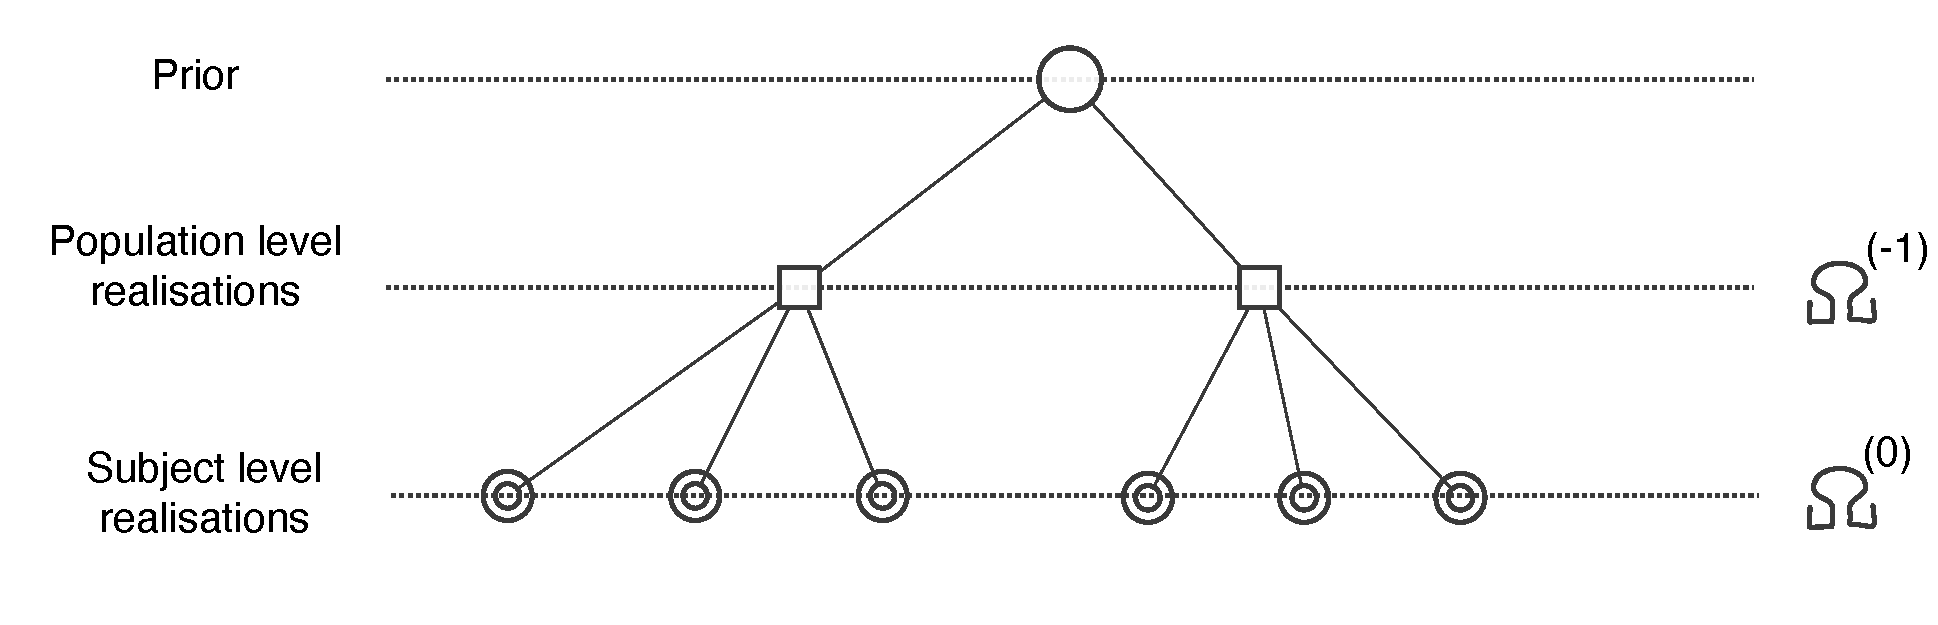
\includegraphics[width=140mm]{pics/IOV0-prior}
\end{tabular}
\caption{Very basic variability structure with prior.}
\label{fig:insulinData}
\end{figure}

\begin{figure}[htb!]
\centering
\begin{tabular}{cc}
 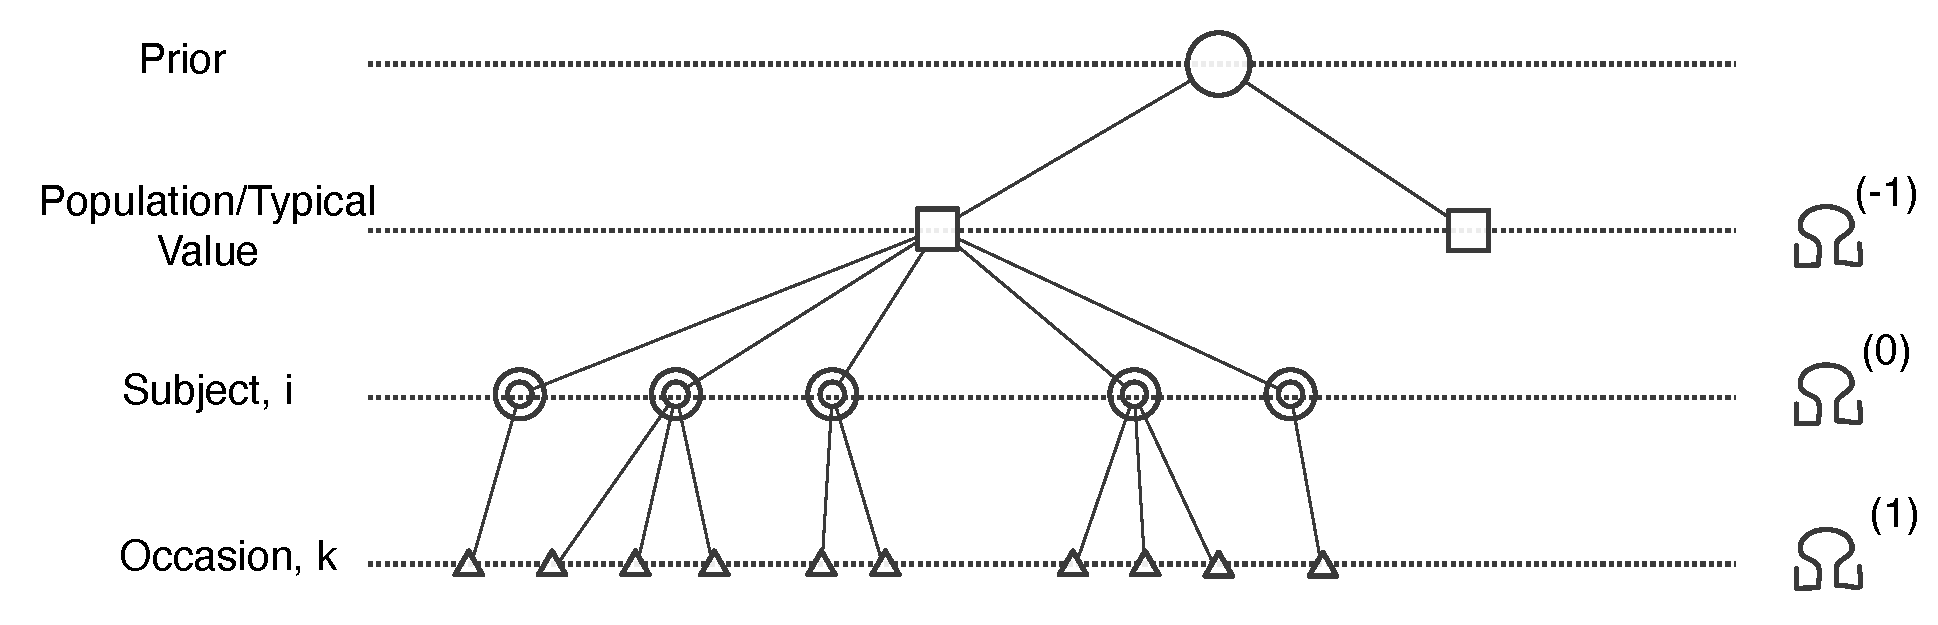
\includegraphics[width=140mm]{pics/IOV_2levels-prior}
\end{tabular}
\caption{Variability structure with IOV and priors on population parameters.}
\label{fig:insulinData}
\end{figure}

\section{New features}
-- prior on any parameter in the model can be defined\\
-- Inverse Wishart -- not supported in UncertML\\
-- basic matrix operators -- inverse, transpose, trace\\
\lstset{language=XML}
\begin{lstlisting}
            <PopulationParameter symbId="lPOP">
                <ct:VariabilityReference>
                    <ct:SymbRef symbIdRef="pop" blkIdRef="vm1"/>
                </ct:VariabilityReference>
                <Distribution>
                    <ProbOnto>
                        <DistributionName>MultivariateNormal2</DistributionName>
                        <Parameter order="1">
                            <ct:Assign>
                                <ct:SymbRef symbIdRef="lMU"/>
                            </ct:Assign>
                        </Parameter>
                        <Parameter order="2">
                            <ct:Assign>
                                <math:Equation>
                                    <math:MatrixUniop op="inverse">
                                        <ct:SymbRef symbIdRef="SIGMA"/>
                                    </math:MatrixUniop>
                                </math:Equation>
                            </ct:Assign>
                        </Parameter>
                    </ProbOnto>
                </Distribution>
            </PopulationParameter>
\end{lstlisting}



%%%%%%%%%%%%%%%%%%%%%%%%%%%%%%%%%%%%%%%%%%%%%%%%%%%%%%%%%%%%%%%%%%%%%%
%%%%%%%%%%%%%%%%%%%%%%%%%%%%%%%%%%%%%%%%%%%%%%%%%%%%%%%%%%%%%%%%%%%%%%%
%%%%%%%%%%%%%%%%%%%%%%%%%%%%%%%%%%%%%%%%%%%%%%%%%%%%%%%%%%%%%%%%%%%%%%%
%%%%%%%%%%%%%%%%%%%%%%%%%%%%%%%%%%%%%%%%%%%%%%%%%%%%%%%%%%%%%%%%%%%%%%%
\chapter{Design -- redesigned}
\label{ch:Design}

%%%%%%%%%%%%%%%%%%%%%%%%%%%%%%%%%%%%%%%%%%%%%%%%%%%%%%%%%%%%%%%%%%%%%%
\section{Design in PharmML $\leq$ 0.6}
Since version 0.2 PharmML was using a CDISC standard, SDM-XML \cite{CDISC:2011a}, 
based trial design. With the commence of the activities of a group working on trial design
for MDL it became clear that this structure is insufficient and had to be reorganised and 
redesigned. Here few reasons 
\begin{itemize}
\item
CDISC based design is missing many element, the most important ones being 
the observations and design spaces. Although the former were supported in 
PharmML, their implementation had not only to be done in another section but 
it also lacked the connectivity to study arms.
\item
number of typical design features, such as arm size, number of arms, total size,
number of samples, number of times, cost function, total cost, was not counted for.
\item
the quite rigid structure with epochs/cells/segment was unfamiliar to modellers 
who prefer a more flexible arm based structure
\item
specifically required for optimal design purposes, the re-definition of covariate model was not 
supported 
\item
design elements were spread over two sections, \xelem{TrialDesing} and \xelem{ModellingSteps}
which created an inconsistent structure
\item
the specification of external datasets, located in \xelem{ModellingSteps}, as the source 
for design belongs to trial design section 
\item
\xelem{ModellingSteps} section should contain only task description 
%- Separation between model-design-tasks required - in Steps only task description - with 2 new elements
\item
the lack of compatibility with the new MDL design proposal -- translation would be 
very hard to achieve given two quite different structures
\end{itemize}
The new design elevates the above issues and because it was developed with both MDL 
and PharmML in mind, it promises a very high \marginpar{\HandCuffLeft} 
degree of compatibility between these two languages -- to be verified during the coming months. 


%%%%%%%%%%%%%%%%%%%%%%%%%%%%%%%%%%%%%%%%%%%%%%%%%%%%%%%%%%%%%%%%%%%%%%
\section{Modifications and extensions}
The new trial design structure consists of
\begin{itemize}
\item
core structure based on the design elements developed for MDL, \cite{Commets2015, CommetsExamples2015}.
\item
and few additional features available in PharmML since 0.2.1 such as individual 
observations, dosing, covariates.
\end{itemize}
While the detailed design is described in detail in the according specification, 
\cite{Commets2015}, the comparison on the following page visualises the changes
and differences. Left, the PharmML $\leq$ 0.6 design elements are shown, distributed
over two sections, \xelem{TrialDesing} and \xelem{ModellingSteps}. 
On the right hand, a detailed list of current elements available for the trial design is given.

All examples provided in the 'Modelling Description Language. Design elements - Examples' 
\cite{CommetsExamples2015} have been successfully implemented.

%\LTcapwidth=\textwidth
%\begin{center}
%\renewcommand{\arraystretch}{1.1}%
%\begin{longtable}{llcccc}
%  \hline
%  \hline
%0.6 & 0.7\\
%%\multicolumn{1}{c}{0.2}			& risation		&  3.0			& 1.4		& 4.3	& 7.3 \\
%  \hline
%
%  \hline \\
%\caption{Structure comparison of the trial design related features.}
%\label{Tab:NewOldDesign}
%%\vspace{-3.5em}
%\end{longtable}
%\end{center}


%%%%% LEFT PAGE %%%%%
\begin{minipage}{0.35\textwidth}
\centering 
\pml $\le$ 0.6\\
\xelem{TrialDesign}
\begin{flushleft} 
\begin{itemize}
\item 
Structure
\begin{itemize}
\item
Arm
\item
Cell
\item
Epoch
\item
Segment
\item
Activity
\begin{itemize}
\item
Bolus
\item
Infusion
\item
Washout
\item
Lookup table
\item
Epoch Ref/Period
\end{itemize}
\end{itemize}
\item
Population
\begin{itemize}
\item
Demographics
\end{itemize}
\item 
Individual Dosing
\end{itemize}
\vspace{2em}
\end{flushleft}
\centering 
\xelem{ModellingSteps}
\begin{flushleft} 
\begin{itemize}
\item 
\textbf{ExternalDataSet}
\item 
Simulation Step
\begin{itemize}
\item 
\textbf{Observations}
\item 
Operation
\end{itemize}
\item 
Estimation Step
\begin{itemize}
\item 
\textbf{ObjectiveData}
\item 
Parameter Estimation
\item 
Operation
\end{itemize}
\end{itemize}
\end{flushleft}
\end{minipage}
%%%%% RIGHT PAGE %%%%%
\begin{minipage}{0.6\textwidth}
\centering 
\pml 0.7\\
\xelem{TrialDesign}
\begin{flushright}
\begin{itemize}
\item 
ExternalDataSet
\item 
Interventions
\begin{itemize}
\item 
Administration
\begin{itemize}
\item 
InterventionRef
\item
Bolus
\item
Infusion
\end{itemize}
\item 
IndividualAdministration
\item 
Action -- Washout
\begin{itemize}
\item 
full reset
\item 
variable-wise
\end{itemize}
\item
InterventionsCombination
\end{itemize}
\item 
Observations
\begin{itemize}
\item 
LookupTable
\item 
IndividualObservations
\item 
Observation
\item 
ObservationsCombination
\end{itemize}
\item 
Covariates
\begin{itemize}
\item 
CovariateModel
\begin{itemize}
\item
Categorical/Category: Probability, OccasionRef, InterventionRef, InterventionSequence
\end{itemize}
\item 
IndividualCovariates
\end{itemize}
\item 
Occasions/OccasionList
\begin{itemize}
\item 
VariabilityReference
\item 
Occasion
\end{itemize}
\item 
Arms
\begin{itemize}
\item 
Simple elements: ArmSize, CostFunction, NumberArms, NumberSamples, NumberTimes, SameTimes, TotalCost, TotalSize
\item 
Arm
\begin{itemize}
\item 
Simple elements: ArmSize, NumberSamples, NumberTimes, SameTimes
\item 
InterventionSequence/List
\item 
ObservationSequence/List
\item 
OccasionSequence/List
\end{itemize}
\end{itemize}
\item 
DesignSpaces
\begin{itemize}
\item 
References: InterventionRef, ObservationRef, ArmRef, SymbRef, CovariateModelRef \& CovariateRef
\item 
Simple elements: ArmSize, DoseAmount, DosingTimes, Duration, NumberArms, NumberSamples, NumberTimes, SampleTimes
\end{itemize}
\end{itemize}
\end{flushright}
\end{minipage}


%%%%%%%%%%%%%%%%%%%%%%%%%%%%%%%%%%%%%%%%%%%%%%%%%%%%%%%%%%%%%%%%%%%%%%%
%\section{Features}
%-- design without arms doable - just dosing and observations\\
%-- old design supported Individual Dosing but now 
%arm-wise scaling is possible as well \\
%-- using parameters in design - 
%\lstset{language=XML}
%\begin{lstlisting}
%                <DesignSpace>
%                    <ct:SymbRef symbIdRef="armSize1"/>
%                    <ct:SymbRef symbIdRef="armSize2"/>
%                    <ct:SymbRef symbIdRef="armSize3"/>
%                    <ct:SymbRef symbIdRef="armSize4"/>
%                    <ct:Assign>
%\end{lstlisting}
%-- new Range element
%\lstset{language=XML}
%\begin{lstlisting}
%                    <DosingTimes>
%                        <ct:Assign>
%                            <ct:Interval>
%                                <ct:LeftEndpoint>
%                                    <ct:Real>0</ct:Real>
%                                </ct:LeftEndpoint>
%                                <ct:RightEndpoint>
%                                    <ct:Real>48</ct:Real>
%                                </ct:RightEndpoint>
%                            </ct:Interval>
%                        </ct:Assign>
%                    </DosingTimes>
%\end{lstlisting}
%-- multiple references possible
%\lstset{language=XML}
%\begin{lstlisting}
%            <DesignSpaces>
%                <DesignSpace>
%                    <InterventionRef oidRef="d1"/>
%                    <InterventionRef oidRef="d2"/>
%                    <DoseAmount>
%\end{lstlisting}
%-- Washout/reset options
%\lstset{language=XML}
%\begin{lstlisting}
%                <Action oid="sd">
%                    <Washout>
%                        <VariableToReset>
%                            <ct:SymbRef symbIdRef="ds"/>
%                            <ResetValue></ResetValue>
%                            <ResetTime></ResetTime>
%                        </VariableToReset>
%                    </Washout>
%                </Action>
%\end{lstlisting}
%-- if IndividualObservations used -- no need to define ObservationSequence etc in the arms, 
%as it is clear from the table where which patient is located\\
%-- reference to observation data not required
%\lstset{language=XML}
%\begin{lstlisting}
%            <ObservationsReference>
%                <ct:OidRef oidRef="OBSoid"/>
%            </ObservationsReference>
%\end{lstlisting}
%
%
%%%%%%%%%%%%%%%%%%%%%%%%%%%%%%%%%%%%%%%%%%%%%%%%%%%%%%%%%%%%%%%%%%%%%%%
%\section{OTHERS}
%
%\begin{itemize}
%\item
%NEW StandardAssignType - DISCUSS!!!!
%\end{itemize}
%

%%%%%%%%%%%%%%%%%%%%%%%%%%%%%%%%%%%%%%%%%%%%%%%%%%%%%%%%%%%%%%%%%%%%%%
%%%%%%%%%%%%%%%%%%%%%%%%%%%%%%%%%%%%%%%%%%%%%%%%%%%%%%%%%%%%%%%%%%%%%%%
%%%%%%%%%%%%%%%%%%%%%%%%%%%%%%%%%%%%%%%%%%%%%%%%%%%%%%%%%%%%%%%%%%%%%%%
%%%%%%%%%%%%%%%%%%%%%%%%%%%%%%%%%%%%%%%%%%%%%%%%%%%%%%%%%%%%%%%%%%%%%%%
\chapter{Other changes}
\label{ch:otherChanges}

%%%%%%%%%%%%%%%%%%%%%%%%%%%%%%%%%%%%%%%%%%%%%%%%%%%%%%%%%%%%%%%%%%%%%%
\section{Box-Cox transformation}
\label{sec:BoxCoxTrafo}
The Box-Cox Transformation \cite{BoxCox:1964} is used to transform data to an approximate normal distribution
and reads
\begin{align}
x^{(\lambda)} = \left\{ \begin{array}{rcl}  \frac{x^{\lambda} -1}{\lambda} & \mbox{for} & \lambda \neq 0 \\  \log(x) & \mbox{for} & \lambda = 0 \end{array}\right. \nonumber
\end{align}
and can be applied to parameters, observations and covariates. 
A random variable, $X$, upon application of the Box-Cox transformation, 
\begin{align*}
        X^{(\lambda)} \sim \mathcal N (X_{typical}^{(\lambda)},\omega^2)
\end{align*}
is called power-normally distributed, i.e.
$X^{(\lambda)}$ has a (truncated) normal distribution with mean $\mu$ and variance $\omega^2$ \cite{LavielleBook:2014}.

\subsection{Box-Cox in parameter model}
A parameter distributed accoring to power-normal distribution reads
\begin{align*}
        V_i^{(\lambda)} \sim \mathcal N (V_{pop}^{(\lambda)},\omega_V^2)
\end{align*}
and can be implemented in PharmML as
\lstset{language=XML}
\begin{lstlisting}
            <IndividualParameter symbId="V">
                <StructuredModel>
                    <Transformation type="BoxCox">
                        <Lambda>
                            <ct:Assign>
                                <ct:SymbRef symbIdRef="lambda"/>
                            </ct:Assign>
                        </Lambda>
                    </Transformation>
                    <LinearCovariate>
                        <PopulationValue>
                            <ct:Assign>
                                <ct:SymbRef symbIdRef="pop_V"/>
                            </ct:Assign>
                        </PopulationValue>
                        <Covariate>
                            <ct:SymbRef blkIdRef="cm1" symbIdRef="logW70"/>
                            <FixedEffect>
                                <ct:SymbRef symbIdRef="beta_V"/>
                            </FixedEffect>
                        </Covariate>
                    </LinearCovariate>
                    <RandomEffects>
                        <ct:SymbRef symbIdRef="eta_V"/>
                    </RandomEffects>
                </StructuredModel>
            </IndividualParameter>
\end{lstlisting}
Note the new attribute value \xatt{BoxCox} and the additional element \xelem{Lambda} 
where the Box-Cox parameter is defined. The rest follows the pattern for the 
\xelem{StructurelModel}.

\subsection{Box-Cox in observation model}
\begin{align*}
        Cc_{obs}^{(\lambda)} = Cc^{(\lambda)} + a \epsilon, \quad \text{with} \quad \epsilon \sim N(0,1)
\end{align*}

\lstset{language=XML}
\begin{lstlisting}
                <Standard symbId="Cc_obs">
                    <Transformation type="BoxCox">
                        <Lambda>
                            <ct:Assign>
                                <ct:SymbRef symbIdRef="lambda"/>
                            </ct:Assign>
                        </Lambda>
                    </Transformation>
                    <Output>
                        <ct:SymbRef blkIdRef="sm1" symbIdRef="Cc"/>
                    </Output>
                    <ErrorModel>
                        <ct:Assign>
                            <ct:SymbRef symbIdRef="a"/>
                        </ct:Assign>
                    </ErrorModel>
                    <ResidualError>
                        <ct:SymbRef symbIdRef="epsilon_Cc"/>
                    </ResidualError>
                </Standard>
\end{lstlisting}


\subsection{Box-Cox in covariate model}
The encoding of the Box-Cox transformation is already possible using the
standard \xelem{FunctionDefinition} element and for now no new structure has been introduced.

%%%%%%%%%%%%%%%%%%%%%%%%%%%%%%%%%%%%%%%%%%%%%%%%%%%%%%%%%%%%%%%%
\section{Encoding of Missing data}
Following discussion at Pavia meeting November 2013, described in the meeting 
report \cite{Swat:2013pavia}, and later comments, it is proposed to extend 
PharmML wrt encoding of data records and to provide means to encode missing 
data using among other standard R (see \href{https://stat.ethz.ch/R-manual/R-devel/library/base/html/is.finite.html}{is.finite\{base\}}) 
and SAS (see \href{http://support.sas.com/documentation/cdl/en/imlug/63541/HTML/default/viewer.htm#imlug_r_sect019.htm}{SAS/IML(R) 9.22}) symbols for special numerical values\footnote{Other possible codes are 
\textbf{DEE} or \textbf{-99} (SAS) -- data entry error or \textbf{SRA} or \textbf{-999} (SAS) 
-- subject refused answer, but will not be introduced unless required}:
\begin{itemize}
\item
\textbf{NA} -- not available/missing data, \xelem{NA}
\item
\textbf{NaN} -- not a number -- impossible values (e.g., dividing by zero), \xelem{NaN}
\item
\textbf{+Inf}/\textbf{-Inf}  -- positive/negative infinity, \xelem{plusInf} and \xelem{minusInf}
\item
\textbf{BLQ}/\textbf{ALQ} -- bellow/above level of quantification\footnote{\textbf{L/H} -- symbols used in dataset in ADAPT5, \cite{DArgenio:2009aa}}, \xelem{BLQ} and \xelem{ALQ}
\end{itemize}
The following hypothetical dataset with several missing DV values
\begin{table}[htdp]
\begin{center}
\small
\renewcommand{\arraystretch}{1.1}% 
\begin{tabular}{rrr}
\hline
ID 	& TIME	& DV	 \\ 
\hline
1 	& 3.43 		& NA 	\\ 
1 	& 5.2 		& 48.03 	 \\ 
1 	& 42.13 		& BLQ	 \\ 
1 	& 52.63 		& $+\infty$ 	 \\ 
1 	& 57.53 		& 72.3  \\ 
...	& ...		& ...	\\ 
\hline
\end{tabular}
\end{center}
\vspace{-1em}\caption{A dataset with examples of missing data.}
\label{tab:uslessDataSet}
\end{table}%

could be encoded in PharmML as the following snippet shows
\lstset{language=XML}
\begin{lstlisting}
    <Definition>
        <Column columnId="ID" columnType="id" valueType="id" columnNum="1"/>
        <Column columnId="TIME" columnType="idv" valueType="real" columnNum="2"/>
        <Column columnId="DV" columnType="dv" valueType="real" columnNum="3"/>
    </Definition>
    <Table>
        <!-- SUBJECT 1 -->
        <Row><ct:Id>i1</ct:Id><ct:Real>3.43</ct:Real><ct:NA/></Row>
        <Row><ct:Id>i1</ct:Id><ct:Real>5.3</ct:Real><ct:Real>48.03</ct:Real></Row> 
        <Row><ct:Id>i1</ct:Id><ct:Real>42.13</ct:Real><ct:BLQ/></Row>
        <Row><ct:Id>i1</ct:Id><ct:Real>52.63</ct:Real><ct:plusInf/></Row>
        <Row><ct:Id>i1</ct:Id><ct:Real>57.53</ct:Real><ct:Real>72.3</ct:Real></Row>
\end{lstlisting}
using the above defined elements.


%%%%%%%%%%%%%%%%%%%%%%%%%%%%%%%%%%%%%%%%%%%%%%%%%%%%%%%%%%%%%%%%%%%%%%
\section{Conditional distributions}

\begin{align}
P(WT|SEX) = 
\left\{ \begin{array}{rcl}     
\mathcal N \big(WT^F_{mean}, WT^F_{variance}\big) & \mbox{for} & SEX == F \\  
\mathcal N \big(WT^M_{mean}, WT^M_{variance}\big) & \mbox{for} & SEX == M
\end{array}\right. \nonumber
\end{align}

\lstset{language=XML}
\begin{lstlisting}
    <CovariateModel blkId="cm1">
        <mdef:Covariate symbId="SEX">
            <mdef:Categorical>
                <mdef:Category catId="M"/>
                <mdef:Category catId="F"/>
            </mdef:Categorical>
        </mdef:Covariate>
        
        <!-- BW distributed conditionally on SEX -->
        <mdef:Covariate symbId="WT">  
            <mdef:Continuous>
                <mdef:Distribution>
                    <mdef:Piecewise>
                        <Piece xmlns="http://www.pharmml.org/pharmml/0.6/Maths">
                            <ProbOnto>
                                <mdef:DistributionName>Normal1</mdef:DistributionName>
                                <mdef:Parameter order="1">
                                    <ct:Assign>
                                        <ct:SymbRef symbIdRef="WT_F_mean"/>
                                    </ct:Assign>
                                </mdef:Parameter>
                                <mdef:Parameter order="2">
                                    <ct:Assign>
                                        <ct:SymbRef symbIdRef="WT_F_variance"/>
                                    </ct:Assign>
                                </mdef:Parameter>
                            </ProbOnto>
                            <Condition>
                                <!-- SEX=="M" -->
                                <LogicBinop op="eq">
                                    <ct:SymbRef blkIdRef="cm1" symbIdRef="SEX"/>
                                    <ct:CatRef catIdRef="M"/>
                                </LogicBinop>
                            </Condition>
                        </Piece>
                        <Piece xmlns="http://www.pharmml.org/pharmml/0.6/Maths">
                            <ProbOnto>
                                <mdef:DistributionName>Normal1</mdef:DistributionName>
                                <mdef:Parameter order="1">
                                    <ct:Assign>
                                        <ct:SymbRef symbIdRef="WT_M_mean"/>
                                    </ct:Assign>
                                </mdef:Parameter>
                                <mdef:Parameter order="2">
                                    <ct:Assign>
                                        <ct:SymbRef symbIdRef="WT_M_variance"/>
                                    </ct:Assign>
                                </mdef:Parameter>
                            </ProbOnto>
                            <Condition>
                                <!-- SEX=="F" -->
                                <LogicBinop op="eq">
                                    <ct:SymbRef blkIdRef="cm1" symbIdRef="SEX"/>
                                    <ct:CatRef catIdRef="F"/>
                                </LogicBinop>
                            </Condition>
                        </Piece>
                    </mdef:Piecewise>
                </mdef:Distribution>
            </mdef:Continuous>
        </mdef:Covariate>
    </CovariateModel>
    \end{lstlisting}


\subsection{Minor changes/extentions}

\begin{itemize}
\item 
\xelem{NumberCounts} NEW
\item 
added several \xatt{columnType} attribute values to be used in SO, such as
'indivParameter', 'popParameter', 'randEffect', 'residual', 'shrinkage'
\item
4. 
NEW StandardAssignType - DISCUSS!!!!
removed
- StandardTripletType
- StandardDupletType
\end{itemize}
\subsection{bugs fixing}

\begin{itemize}
\item 
correct sm1 to sm12 etc. in PKL macro examples!
\item 

\end{itemize}


- Distribution element for discrete data models???\\


\appendix
\chapter{Selected distributions in ProbOnto}
\label{ch:probontoAppendix}

The full first version of ProbOnto will be released very soon. We provide 
here a brief overview of its content with the most relevant distributions 
currently required for the DDMoRe use cases. 


%\chapter{Application of selected distributions}
%\label{ch:distributions}
%
%
%%%%%%%%%%%%%%%%%%%%%%%%%%%%%%%%%%%%%%%%%%%%%%%%%%%%%%%%%%%%%%%%%%%%%%%
%\section{Binomial Distribution}
%\url{http://wwwpub.utdallas.edu/~scniu/}
%\begin{itemize}
%\item 
%The number of heads/tails in a sequence of coin flips
%\item
%Vote counts for two different candidates in an election
%\item
%The number of male/female employees in a company
%\item
%The number of accounts that are in compliance or not
%in compliance with an accounting procedure
%\item
%The number of successful sales calls
%\item
%The number of defective products in a production run
%\item
%The number of days in a month your company's computer
%network experiences a problem
%\end{itemize}
%
%%%%%%%%%%%%%%%%%%%%%%%%%%%%%%%%%%%%%%%%%%%%%%%%%%%%%%%%%%%%%%%%%%%%%%%
%\section{Poisson Distribution}
%\url{http://wwwpub.utdallas.edu/~scniu/}
%\begin{itemize}
%\item
%The hourly number of customers arriving at a bank
%\item
%The daily number of accidents on a particular stretch
%of highway
%\item
%The hourly number of accesses to a particular web
%server
%\item
%The daily number of emergency calls in Dallas
%\item
%The number of typos in a book
%\item
%The monthly number of employees who had an absence
%in a large company
%\item
%Monthly demands for a particular product
%\end{itemize}
%\url{https://en.wikipedia.org/wiki/Poisson_distribution#History}
%\begin{itemize}
%\item
%number of soldiers killed accidentally by horse kicks
%\end{itemize}
%

\bibliographystyle{plain}
\bibliography{pharmml-specification}
\end{document}





%TEMPLATES 
%% 1. Template for table with figures
%\begin{figure}[htbp]
%\centering
%\begin{tabular}{cc}
% \includegraphics[width=80mm]{pics/pic1} & 
% \includegraphics[width=80mm]{pics/pic2} \\
% \includegraphics[width=80mm]{pics/pic3} &
% \includegraphics[width=80mm]{pics/pic4}
%\end{tabular}
%\caption{about the figure}
%\label{figTable:labelText}
%\end{figure}

%\begin{table}[ht]
%\begin{center}
%\begin{tabular}{rrrrrrrrrrr}
%  \hline
% & 1 & 2 & 3 & 4 & 5 & 6 & 7 & 8 & 9 & 10 \\ 
%  \hline
%1 & 0.24 & -1.47 & -0.56 & 0.24 & 0.71 & 1.23 & 0.44 & 0.40 & 1.10 & 1.84 \\ 
%   \hline
%\end{tabular}
%\end{center}
%\end{table}
 

%\begin{figure}[htb!]
%\centering
%  \includegraphics[width=105mm]{}
% \caption{}
% \label{fig:myplot}
%\end{figure}

%PIECE-WISE
%f(z) =     \left\{ \begin{array}{rcl}
%         value1 & \mbox{for} & condition1 \\ 
%         value1 & \mbox{for} & condition1
%             \end{array}\right.


%%%%%%%%%%%%%%%%%%%%%%%%%%%%%%%%%%%%%%%%%%%%%%%%%%
% FOR LOOPS and GRUENENTHAL MODEL
%%%%%%%%%%%%%%%%%%%%%%%%%%%%%%%%%%%%%%%%%%%%%%%%%%
%%%%%%%%%%%%%%%%%%%%%%%%%%%%%%%%%%%%%%%%%%%%%%%%%%

%\subsection{For loops for categorical models}
%Loops make implementation of model simpler, especially when multiple categories have to be considered.
%Following ordered categorical model for NRS pain score, based on \cite{Wang:2014}, 
%\begin{align}
%& \text{for j = 1 to m} \nonumber \\
%  & \quad logit( P(PS <= cat_j) ) = \sum_{k=0}^{m} \beta_k + \theta_{base}(PS(t=0)-4.2) + fp(t) + f(drug) \nonumber \\ 
%& \text{end} \nonumber
%\end{align}
%has been implemented using a for-loop as the following code for the observation model shows. Note that 
%model parameters to be estimated and categories have been formulated as vectors, $\beta$ and $categoryVector$,
%respectively. Compared to the original formulation, see Figure \ref{fig:GruenenthalModel}, the subject 
%index \emph{i} of the observation variable $PS$ has been omitted.
%\lstset{language=XML}
%\begin{lstlisting}
%<ObservationModel blkId="om1">
%    <Discrete>
%        <CategoricalData>
%            <SimpleParameter symbId="m"/>
%            <SimpleParameter symbId="beta">
%                <ct:Assign>
%                    <ct:Vector>
%                        <ct:VectorElements>
%                            <ct:SymbRef blkIdRef="pm1" symbIdRef="beta_1"/>
%                            <!-- omitted beta_2 .. beta_{m-1} -->
%                            <ct:SymbRef blkIdRef="pm1" symbIdRef="beta_m"/>
%                        </ct:VectorElements>
%                    </ct:Vector>
%                </ct:Assign>
%            </SimpleParameter>
%            
%            <SimpleParameter symbId="categoryVector">
%                <ct:Assign>
%                    <ct:Vector>
%                        <ct:VectorElements>
%                            <ct:SymbRef symbIdRef="cat1"/>
%                            <!-- omitted cat_1 ... cat_{m-1} -->
%                            <ct:SymbRef symbIdRef="catm"/>
%                        </ct:VectorElements>
%                    </ct:Vector>
%                </ct:Assign>
%            </SimpleParameter>
%            
%            <ct:Variable symbolType="int" symbId="i"/>
%            <ct:Variable symbolType="int" symbId="j"/>
%            <ct:Variable symbolType="int" symbId="k"/>
%            
%            <ListOfCategories> 
%                <Category symbId="cat0"/>
%                <!-- omitted other categories -->
%                <Category symbId="catm"/>
%            </ListOfCategories>
%            
%            <CategoryVariable symbId="PS"/>
%
%        <!-- 
%        for j=1 to m
%          logit(P(PS_j<=cat_j))=\Sigma_{k=0}^{m}beta_k+theta_base*(PS_0-4.2)+fp(t)+f(drug) 
%        end 
%        -->
%            <ForLoop>
%                <ct:ProbabilityAssignment>
%                    <Probability linkFunction="logit">
%                        <math:LogicBinop op="leq">
%                            <ct:SymbRef symbIdRef="PS"/>
%                            <ct:VectorSelector>
%                                <ct:SymbRef symbIdRef="categoryVector"/>
%                                <ct:Cell>
%                                    <ct:SymbRef symbIdRef="j"/>
%                                </ct:Cell>
%                            </ct:VectorSelector>
%                        </math:LogicBinop>
%                    </Probability>
%                    <ct:Assign>
%                        <math:Equation>
%                            <math:Binop op="plus">
%                                <math:Binop op="plus">
%                                    <math:Binop op="plus">
%                                        <ct:Sum>
%                                            <math:Equation>
%                                                <ct:VectorSelector>
%                                                    <ct:SymbRef symbIdRef="beta"/>
%                                                    <ct:Cell>
%                                                        <ct:SymbRef symbIdRef="k"/>
%                                                    </ct:Cell>
%                                                </ct:VectorSelector>
%                                            </math:Equation>
%                                            <ct:SumIndex>
%                                                <ct:SymbRef symbIdRef="k"/>
%                                            </ct:SumIndex>
%                                            <ct:LowLimit>
%                                                <ct:Int>0</ct:Int>
%                                            </ct:LowLimit>
%                                            <ct:UpLimit>
%                                                <ct:SymbRef symbIdRef="m"/>
%                                            </ct:UpLimit>
%                                        </ct:Sum>
%                                        <math:Binop op="times">
%                                            <ct:SymbRef symbIdRef="theta_base"/>
%                                            <math:Binop op="minus">
%                                                <ct:VectorSelector>
%                                                    <ct:SymbRef symbIdRef="PS"/>
%                                                    <ct:Cell>
%                                                        <ct:Int>0</ct:Int>
%                                                    </ct:Cell>
%                                                </ct:VectorSelector>
%                                                <ct:Real>4.2</ct:Real>
%                                            </math:Binop>
%                                        </math:Binop>
%                                    </math:Binop>
%                                    <!-- function fp(t) -->
%                                    <math:FunctionCall>
%                                        <ct:SymbRef symbIdRef="fp"/>
%                                        <math:FunctionArgument symbId="p_max">
%                                            <ct:SymbRef blkIdRef="pm1" symbIdRef="Pmax"/>
%                                        </math:FunctionArgument>
%                                        <math:FunctionArgument symbId="k_plc">
%                                            <ct:SymbRef blkIdRef="pm1" symbIdRef="Kplc"/>
%                                        </math:FunctionArgument>
%                                        <math:FunctionArgument symbId="time">
%                                            <ct:SymbRef symbIdRef="t"/>
%                                        </math:FunctionArgument>
%                                    </math:FunctionCall>
%                                </math:Binop>
%                                <!-- function f(drug) -->
%                                <math:Binop op="divide">
%                                    <math:Binop op="times">
%                                        <ct:SymbRef blkIdRef="pm1" symbIdRef="Emax"/>
%                                        <ct:SymbRef blkIdRef="sm1" symbIdRef="C_M"/>
%                                    </math:Binop>
%                                    <math:Binop op="plus">
%                                        <ct:SymbRef blkIdRef="pm1" symbIdRef="EC50"/>
%                                        <ct:SymbRef blkIdRef="sm1" symbIdRef="C_M"/>
%                                    </math:Binop>
%                                </math:Binop>
%                            </math:Binop>
%                        </math:Equation>
%                    </ct:Assign>
%                </ct:ProbabilityAssignment>
%                <ct:LoopIndex>
%                    <ct:SymbRef symbIdRef="j"/>
%                </ct:LoopIndex>
%                <ct:StartIndex>
%                    <ct:Int>1</ct:Int>
%                </ct:StartIndex>
%                <ct:EndIndex>
%                    <ct:SymbRef symbIdRef="m"/>
%                </ct:EndIndex>
%            </ForLoop>
%        </CategoricalData>
%    </Discrete>
%</ObservationModel>
%\end{lstlisting}
%The full model is provided in the example folder as \emph{categorical\_GruenenthalModel.xml}
%
%
%\begin{figure}[htb!]
%\centering
%  \includegraphics[width=40mm,angle=-90]{pics/CategoricalWithSumModel.jpg}
% \caption{}
% \label{fig:GruenenthalModel}
%\end{figure}
